\chapter{\FPUChapterName}
\label{sec:FPU}

\newcommand{\FNURLSTACK}{\footnote{\href{http://go.yurichev.com/17123}{wikipedia.org/wiki/Stack\_machine}}}
\newcommand{\FNURLFORTH}{\footnote{\href{http://go.yurichev.com/17124}{wikipedia.org/wiki/Forth\_(programming\_language)}}}
\newcommand{\FNURLIEEE}{\footnote{\href{http://go.yurichev.com/17125}{wikipedia.org/wiki/IEEE\_floating\_point}}}
\newcommand{\FNURLSP}{\footnote{\href{http://go.yurichev.com/17126}{wikipedia.org/wiki/Single-precision\_floating-point\_format}}}
\newcommand{\FNURLDP}{\footnote{\href{http://go.yurichev.com/17127}{wikipedia.org/wiki/Double-precision\_floating-point\_format}}}
\newcommand{\FNURLEP}{\footnote{\href{http://go.yurichev.com/17128}{wikipedia.org/wiki/Extended\_precision}}}

\RU{\ac{FPU}\EMDASH блок в процессоре работающий с числами с плавающей запятой.}
\EN{The \ac{FPU} is a device within the main \ac{CPU}, specially designed to deal with floating point numbers.}
\RU{Раньше он назывался \q{сопроцессором} и он стоит немного в стороне от \ac{CPU}.}
\EN{It was called \q{coprocessor} in the past and it stays somewhat aside of the main \ac{CPU}.}

\section{IEEE 754}

\RU{Число с плавающей точкой в формате IEEE 754 состоит из \IT{знака}, \IT{мантиссы}\footnote{\IT{significand} или \IT{fraction} 
в англоязычной литературе} и \IT{экспоненты}.}
\EN{A number in the IEEE 754 format consists of a \IT{sign}, a \IT{significand} (also called \IT{fraction}) and an \IT{exponent}.}

\section{x86}

\RU{Перед изучением \ac{FPU} в x86 полезно ознакомиться с тем как работают стековые машины\FNURLSTACK 
или ознакомиться с основами языка Forth\FNURLFORTH.}
\EN{It is worth looking into stack machines\FNURLSTACK or learning the basics of the Forth language\FNURLFORTH,
before studying the \ac{FPU} in x86.}

\index{Intel!80486}
\index{Intel!FPU}
\RU{Интересен факт, что в свое время (до 80486) сопроцессор был отдельным чипом на материнской плате, 
и вследствие его высокой цены, он не всегда присутствовал. Его можно было докупить и установить отдельно}%
\EN{It is interesting to know that in the past (before the 80486 CPU) the coprocessor was a separate chip 
and it was not always pre-installed on the motherboard. It was possible to buy it separately and install it}%
\footnote{\RU{Например, Джон Кармак использовал в своей игре Doom числа с фиксированной запятой 
% TODO FIXME link does not work
(\href{http://go.yurichev.com/17357}{ru.wikipedia.org/wiki/Число\_с\_фиксированной\_запятой}), хранящиеся
в обычных 32-битных \ac{GPR} (16 бит на целую часть и 16 на дробную),
чтобы Doom работал на 32-битных компьютерах без FPU, т.е. 80386 и 80486 SX.}
\EN{For example, John Carmack used fixed-point arithmetic 
(\href{http://go.yurichev.com/17356}{wikipedia.org/wiki/Fixed-point\_arithmetic}) values in his Doom video game, stored in 
32-bit \ac{GPR} registers (16 bit for integral part and another 16 bit for fractional part), so Doom
could work on 32-bit computers without FPU, i.e., 80386 and 80486 SX.}}.
\RU{Начиная с 80486 DX в состав процессора всегда входит FPU.}
\EN{Starting with the 80486 DX CPU, the \ac{FPU} is integrated in the \ac{CPU}.}

\index{x86!\Instructions!FWAIT}
\RU{Этот факт может напоминать такой рудимент как наличие инструкции \TT{FWAIT}, 
которая заставляет
\ac{CPU} ожидать, пока \ac{FPU} закончит работу}\EN{The \TT{FWAIT} instruction reminds us of that fact---it
switches the \ac{CPU} to a waiting state, so it can wait until the \ac{FPU} is done with its work}.
\RU{Другой рудимент это тот факт, что опкоды \ac{FPU}-инструкций начинаются с т.н. \q{escape}-опкодов 
(\TT{D8..DF}) как опкоды, передающиеся в отдельный сопроцессор.}
\EN{Another rudiment is the fact that the \ac{FPU} instruction 
opcodes start with the so called \q{escape}-opcodes (\TT{D8..DF}), i.e., 
opcodes passed to a separate coprocessor.}

\index{IEEE 754}
\label{FPU_is_stack}
\RU{FPU имеет стек из восьми 80-битных регистров:}
\EN{The FPU has a stack capable to holding 8 80-bit registers, and each register can hold a number 
in the IEEE 754\FNURLIEEE format.}
\RU{\ST{0}..\ST{7}. Для краткости, IDA и \olly отображают \ST{0} как \TT{ST},
что в некоторых учебниках и документациях означает \q{Stack Top} (\q{вершина стека}).}
\RU{Каждый регистр может содержать число в формате IEEE 754\FNURLIEEE.}
\EN{They are \ST{0}..\ST{7}. For brevity, IDA and \olly show \ST{0} as \TT{ST}, 
which is represented in some textbooks and manuals as \q{Stack Top}.}

\section{ARM, MIPS, x86/x64 SIMD}

\RU{В ARM и MIPS FPU это не стек, а просто набор регистров.}
\EN{In ARM and MIPS the FPU is not a stack, but a set of registers.}
\RU{Такая же идеология применяется в расширениях SIMD в процессорах x86/x64.}
\EN{The same ideology is used in the SIMD extensions of x86/x64 CPUs.}

\section{\CCpp}

\index{float}
\index{double}
\RU{В стандартных \CCpp имеются два типа для работы с числами с плавающей запятой: 
\Tfloat (\IT{число одинарной точности}\FNURLSP, 32 бита)
\footnote{Формат представления float-чисел затрагивается в разделе 
\IT{\WorkingWithFloatAsWithStructSubSubSectionName}~(\myref{sec:floatasstruct}).}
и \Tdouble (\IT{число двойной точности}\FNURLDP, 64 бита).}
\EN{The standard \CCpp languages offer at least two floating number types, \Tfloat (\IT{single-precision}\FNURLSP, 32 bits)
\footnote{the single precision floating point number format is also addressed in 
the \IT{\WorkingWithFloatAsWithStructSubSubSectionName}~(\myref{sec:floatasstruct}) section}
and \Tdouble (\IT{double-precision}\FNURLDP, 64 bits).}

\index{long double}
\RU{GCC также поддерживает тип \IT{long double} (\IT{extended precision}\FNURLEP, 80 бит), но MSVC~--- нет.}
\EN{GCC also supports the \IT{long double} type (\IT{extended precision}\FNURLEP, 80 bit), which MSVC doesn't.}

\RU{Несмотря на то, что \Tfloat занимает столько же места, сколько и \Tint на 32-битной архитектуре, 
представление чисел, разумеется, совершенно другое.}
\EN{The \Tfloat type requires the same number of bits as the \Tint type in 32-bit environments, 
but the number representation is completely different.}

\ifdefined\RUSSIAN
\section{Простой пример}

Рассмотрим простой пример:
\fi

\ifdefined\ENGLISH
\section{Simple example}

Let's consider this simple example:
\fi

\lstinputlisting{patterns/12_FPU/1_simple/simple.c}

\subsectionold{x86}

% subsubsections
\EN{\subsubsection{MSVC}

Compile it in MSVC 2010:

\lstinputlisting[caption=MSVC 2010: \ttf{}]{patterns/12_FPU/1_simple/MSVC_EN.asm}

\FLD takes 8 bytes from stack and loads the number into the \ST{0} register, automatically converting 
it into the internal 80-bit format (\IT{extended precision}).

\myindex{x86!\Instructions!FDIV}

\FDIV divides the value in \ST{0} by the number stored at address 
\GTT{\_\_real@40091eb851eb851f}~---the value 3.14 is encoded there. 
The assembly syntax doesn't support floating point numbers, so 
what we see here is the hexadecimal representation of 3.14 in 64-bit IEEE 754 format.

After the execution of \FDIV \ST{0} holds the \gls{quotient}.

\myindex{x86!\Instructions!FDIVP}

By the way, there is also the \FDIVP instruction, which divides \ST{1} by \ST{0}, 
popping both these values from stack and then pushing the result. 
If you know the Forth language\FNURLFORTH,
you can quickly understand that this is a stack machine\FNURLSTACK.

The subsequent \FLD instruction pushes the value of $b$ into the stack.

After that, the quotient is placed in \ST{1}, and \ST{0} has the value of $b$.

\myindex{x86!\Instructions!FMUL}

The next \FMUL instruction does multiplication: $b$ from \ST{0} is multiplied by by value at 
\GTT{\_\_real@4010666666666666} (the numer 4.1 is there) and leaves the result in the \ST{0} register.

\myindex{x86!\Instructions!FADDP}

The last \FADDP instruction adds the two values at top of stack, storing the result in \ST{1} 
and then popping the value of \ST{0}, thereby leaving the result at the top of the stack, in \ST{0}.

The function must return its result in the \ST{0} register, 
so there are no any other instructions except the function epilogue after \FADDP.

\ifdefined\IncludeOlly
\input{patterns/12_FPU/1_simple/olly_EN.tex}
\fi
}
\RU{\subsubsectionold{MSVC}

Компилируем в MSVC 2010:

\lstinputlisting[caption=MSVC 2010: \ttf{}]{patterns/12_FPU/1_simple/MSVC_RU.asm}

\FLD берет 8 байт из стека и загружает их в регистр \ST{0}, автоматически конвертируя во внутренний 
80-битный формат (\IT{extended precision}).

\myindex{x86!\Instructions!FDIV}
\FDIV делит содержимое регистра \ST{0} на число, лежащее по адресу \GTT{\_\_real@40091eb851eb851f}~--- 
там закодировано значение 3,14. Синтаксис ассемблера не поддерживает подобные числа, 
поэтому мы там видим шестнадцатеричное представление числа 3,14 в формате IEEE 754.

После выполнения \FDIV в \ST{0} остается \glslink{quotient}{частное}.

\myindex{x86!\Instructions!FDIVP}
Кстати, есть ещё инструкция \FDIVP, которая делит \ST{1} на \ST{0}, 
выталкивает эти числа из стека и заталкивает результат. 
Если вы знаете язык Forth\FNURLFORTH, то это как раз оно и есть~--- стековая машина\FNURLSTACK.

Следующая \FLD заталкивает в стек значение $b$.

После этого в \ST{1} перемещается результат деления, а в \ST{0} теперь $b$.

\myindex{x86!\Instructions!FMUL}
Следующий \FMUL умножает $b$ из \ST{0} на значение \GTT{\_\_real@4010666666666666}~--- 
там лежит число 4,1~--- и оставляет результат в \ST{0}.

\myindex{x86!\Instructions!FADDP}
Самая последняя инструкция \FADDP складывает два значения из вершины стека 
в \ST{1} и затем выталкивает значение, лежащее в \ST{0}. 
Таким образом результат сложения остается на вершине стека в \ST{0}.

Функция должна вернуть результат в \ST{0}, так что больше ничего здесь не производится, 
кроме эпилога функции.

\input{patterns/12_FPU/1_simple/olly_RU.tex}
}
\EN{\subsubsectionold{GCC}

GCC 4.4.1 (with \Othree option) emits the same code, just slightly different:

\lstinputlisting[caption=\Optimizing GCC 4.4.1]{patterns/12_FPU/1_simple/GCC_EN.asm}

The difference is that, first of all, 3.14 is pushed to the stack (into \ST{0}), and then the value 
in \GTT{arg\_0} is divided by the value in \ST{0}.

\myindex{x86!\Instructions!FDIVR}

\FDIVR stands for \IT{Reverse Divide}~---to divide with divisor and dividend swapped with each other. 
There is no likewise instruction for multiplication since it is 
a commutative operation, so we just have \FMUL without its \GTT{-R} counterpart.

\myindex{x86!\Instructions!FADDP}

\FADDP adds the two values but also pops one value from the stack. 
After that operation, \ST{0} holds the sum.

}
\RU{\ifdefined\IncludeGCC
\subsubsection{GCC}

GCC 4.4.1 (с опцией \Othree) генерирует похожий код, хотя и с некоторой разницей:

\lstinputlisting[caption=\Optimizing GCC 4.4.1]{patterns/12_FPU/1_simple/GCC_RU.asm}

Разница в том, что в стек сначала заталкивается 3,14 (в \ST{0}), а затем значение 
из \GTT{arg\_0} делится на то, что лежит в регистре \ST{0}.

\myindex{x86!\Instructions!FDIVR}
\FDIVR означает \IT{Reverse Divide}~--- делить, поменяв делитель и делимое местами. 
Точно такой же инструкции для умножения нет, потому что она была бы бессмысленна (ведь умножение 
операция коммутативная), так что остается только \FMUL без соответствующей ей \GTT{-R} инструкции.

\myindex{x86!\Instructions!FADDP}
\FADDP не только складывает два значения, но также и выталкивает из стека одно значение. 
После этого в \ST{0} остается только результат сложения.

\fi
}


\ifdefined\IncludeARM
\subsection{ARM: \OptimizingXcodeIV (\ARMMode)}

\RU{Пока в ARM не было стандартного набора инструкций для работы с плавающей точкой}
\EN{Until ARM has floating standardized point support}, \RU{разные производители процессоров
могли добавлять свои расширения для работы с ними}\EN{several processor manufacturers may add their own 
instructions extensions}.
\RU{Позже, был принят стандарт}\EN{Then, } VFP (\IT{Vector Floating Point})\EN{ was standardized}.

\RU{Важное отличие от x86 в том, что там вы работаете с FPU-стеком, а здесь стека нет, 
здесь вы работаете просто с регистрами.}
\EN{One important difference from x86, there you working with FPU-stack, but here, in ARM, there
are no any stack, you work just with registers.}

\lstinputlisting[label=ARM_leaf_example10]{patterns/12_FPU/1_simple/ARM/Xcode_ARM_O3.asm}

\index{ARM!D-\registers{}}
\index{ARM!S-\registers{}}
\RU{Итак, здесь мы видим использование новых регистров, с префиксом D.}
\EN{So, we see here new registers used, with D prefix.}
\RU{Это 64-битные регистры, их 32, и их можно
использовать и для чисел с плавающей точкой двойной точности (double) и для 
SIMD (в ARM это называется NEON).}
\EN{These are 64-bit registers, there are 32 of them, and these can be used both for floating-point numbers 
(double) but also for SIMD (it is called NEON here in ARM).}
\RU{Имеются также 32 32-битных S-регистра, они применяются для работы с числами 
с плавающей точкой одинарной точности (float).}
\EN{There are also 32 32-bit S-registers, they are intended to be used for single precision 
floating pointer numbers (float).}
\RU{Запомнить легко: D-регистры предназначены для чисел double-точности, 
а S-регистры ~--- для чисел single-точности.}
\EN{It is easy to remember: D-registers are intended for double precision numbers, while
S-registers~---for single precision numbers.}
\RU{Больше об этом}\EN{More about it}: \ref{ARM_VFP_registers}.

\RU{Обе константы}\EN{Both} ($3.14$ \AndENRU $4.1$) \RU{хранятся в памяти в формате IEEE 754.}
\EN{constants are stored in memory in IEEE 754 form.}

\index{ARM!\Instructions!VLDR}
\index{ARM!\Instructions!VMOV}
\RU{Инструкции }\TT{VLDR} \AndENRU \TT{VMOV}
\RU{, как можно догадаться, это аналоги обычных \TT{LDR} и \MOV, но они работают с D-регистрами.}
\EN{instructions, as it can be easily deduced, are analogous to the \TT{LDR} and \MOV instructions,
but they works with D-registers.}
\RU{Важно отметить, что эти инструкции, как и D-регистры, предназначены не только для работы 
с числами с плавающей точкой, но пригодны также и для работы с SIMD (NEON), и позже это также будет видно.}
\EN{It should be noted that these instructions, just like D-registers, are intended not only for
floating point numbers, but can be also used for SIMD (NEON) operations and this will also be revealed soon.}

\RU{Аргументы передаются в функцию обычным путем, через R-регистры, однако, 
каждое число, имеющее двойную точность, занимает 64 бита, так что для передачи каждого нужны два R-регистра.}
\EN{Arguments are passed to function in common way, via R-registers, however,
each number having double precision has size 64-bits, so, for passing each, two R-registers are needed.}

\TT{``VMOV D17, R0, R1''} \RU{в самом начале составляет два 32-битных значения из \Reg{0} и \Reg{1} 
в одно 64-битное и сохраняет в}
\EN{at the very beginning, composing two 32-bit values from \Reg{0} and \Reg{1} into one 64-bit value
and saves it to} \TT{D17}.

\TT{``VMOV R0, R1, D16''} \RU{в конце это обратная процедура}\EN{is inverse operation}, 
\RU{то что было в}\EN{what was in} \TT{D16} 
\RU{остается в двух регистрах}\EN{leaving in two} \Reg{0} \AndENRU \Reg{1}\EN{ registers},
\RU{потому что,}\EN{since} \RU{число с двойной точностью}\EN{double-precision number}, 
\RU{занимающее 64 бита}\EN{needing 64 bits for storage}, \RU{возвращается в паре регистров \Reg{0} и \Reg{1}}
\EN{is returning in the \Reg{0} and \Reg{1} registers pair}.

\index{ARM!\Instructions!VDIV}
\index{ARM!\Instructions!VMUL}
\index{ARM!\Instructions!VADD}
\TT{VDIV}, \TT{VMUL} \AndENRU \TT{VADD}, \RU{это, собственно, инструкции для работы с числами 
с плавающей точкой, вычисляющие, соответственно, \glslink{quotient}{частное}, \glslink{product}{произведение} и сумму.}
\EN{are instruction for floating point numbers processing, computing, \gls{quotient}, 
\gls{product} and sum, respectively.}

\RU{Код для thumb-2 такой же.}\EN{The code for thumb-2 is same.}

\subsection{ARM: \OptimizingKeilVI (\ThumbMode)}

\lstinputlisting{patterns/12_FPU/1_simple/ARM/Keil_O3_thumb.asm}

\RU{Keil компилировал для процессора, в котором может и не быть поддержки FPU или NEON.}
\EN{Keil generated for processor without FPU or NEON support.}
\RU{Так что числа с двойной точностью передаются в парах обычных R-регистров}
\EN{So, double-precision floating numbers are passed via generic R-registers},
\RU{а вместо FPU-инструкций вызываются сервисные библиотечные функции}
\EN{and instead of FPU-instructions, service library functions are called (like}
\TT{\_\_aeabi\_dmul}, \TT{\_\_aeabi\_ddiv}, \TT{\_\_aeabi\_dadd}
\RU{, эмулирующие умножение, деление и сложение чисел с плавающей точкой.}
\EN{) which emulates multiplication, division and addition floating-point numbers.}
\RU{Конечно, это медленнее чем FPU-сопроцессор, но лучше, чем ничего.}
\EN{Of course, that is slower than FPU-coprocessor, but it is better than nothing.}

\RU{Кстати, похожие библиотеки для эмуляции сопроцессорных инструкций были очень распространены в x86, 
когда сопроцессор был редким и дорогим, и стоял далеко не на всех компьютерах.}
\EN{By the way, similar FPU-emulating libraries were very popular in x86 world when coprocessors were rare
and expensive, and were installed only on expensive computers.}

\index{ARM!soft float}
\index{ARM!armel}
\index{ARM!armhf}
\index{ARM!hard float}
\RU{Эмуляция FPU-сопроцессора в ARM называется \IT{soft float} или \IT{armel}, 
а использование FPU-инструкций сопроцессора ~--- \IT{hard float} или \IT{armhf}.}
\EN{FPU-coprocessor emulating called \IT{soft float} or \IT{armel} in ARM world, 
while using coprocessor's FPU-instructions called \IT{hard float} or \IT{armhf}.}

\iffalse
% TODO разобраться...
\index{Raspberry Pi}
\RU{Ядро Linux, например, для Raspberry Pi может поставляться в двух вариантах.}
\EN{For example, Linux kernel for Raspberry Pi is compiled in two variants.}
\RU{В случае \IT{soft float}, аргументы будут передаваться через R-регистры, 
а в случае \IT{hard float}, через D-регистры.}
\EN{In \IT{soft float} case, arguments will be passed via R-registers, and in \IT{hard float} 
case~---via D-registers.}

\RU{И это то, что помешает использовать, например, armhf-библиотеки
из armel-кода или наоборот, поэтому, весь код в дистрибутиве Linux должен быть скомпилирован
в соответствии с выбранным соглашением о вызовах.}
\EN{And that is what do not let you use e.g. armhf-libraries from armel-code or vice versa,
so that is
why all code in Linux distribution must be compiled according to the one chosen calling convention.}
\fi

\subsection{ARM64: \Optimizing GCC (Linaro) 4.9}

\RU{Очень компактный код}\EN{Very compact code}:

\lstinputlisting{patterns/12_FPU/1_simple/ARM/ARM64_GCC_O3.s}

\subsection{ARM64: \NonOptimizing GCC (Linaro) 4.9}

\lstinputlisting{patterns/12_FPU/1_simple/ARM/ARM64_GCC_O0.s}

\NonOptimizing GCC \RU{более многословный}\EN{is more verbose}.
\RU{Здесь много ненужных перетасовок значений, включая явно избыточный код 
(последние две инструкции \TT{GMOV}).}
\EN{There are a lot of unnecessary value shuffling, including clearly redundant code 
(last two \TT{FMOV} instructions).}
\RU{Должно быть}\EN{Probably}, GCC 4.9 \RU{пока еще не очень хорош для генерации кода под ARM64}\EN{is not 
yet good on generating ARM64 code}.
\RU{Вот что интересно заметить, это то что у ARM64 64-битные регистры, и D-регистры так же 64-битные.}
\EN{What is worth to note is that ARM64 has 64-bit registers, and D-registers are 64-bit ones as well.}
\RU{Так что компилятор может сохранять значения типа \Tdouble в \ac{GPR} вместо локального стека.}
\EN{So the compiler is free to save values of \Tdouble type in \ac{GPR}'s instead of local stack.}
\RU{Это не было возможно на 32-битных CPU}\EN{This wasn't possible on 32-bit CPUs}.

\RU{И снова, как упражнение, вы можете попробовать соптимизировать эту ф-цию вручную, без добавления
новых инструкций вроде \TT{FMADD}.}
\EN{And again, as an exercise, you can try to optimize this function manually, without introducing
new instructions like \TT{FMADD}.}

\fi
\ifdefined\IncludeMIPS
\EN{\subsubsection{MIPS}

MIPS can support several coprocessors (up to 4), 
the zeroth of which is a special control coprocessor,
and first coprocessor is the FPU.

As in ARM, the MIPS coprocessor is not a stack machine, it has 32 32-bit registers (\$F0-\$F31):
\myref{MIPS_FPU_registers}.

When one needs to work with 64-bit \Tdouble values, a pair of 32-bit F-registers is used.

\lstinputlisting[caption=\Optimizing GCC 4.4.5 (IDA)]{patterns/12_FPU/1_simple/MIPS_O3_IDA_EN.lst}

The new instructions here are:

\myindex{MIPS!\Instructions!LWC1}
\myindex{MIPS!\Instructions!DIV.D}
\myindex{MIPS!\Instructions!MUL.D}
\myindex{MIPS!\Instructions!ADD.D}
\begin{itemize}

\item \INS{LWC1} loads a 32-bit word into a register of the first coprocessor (hence \q{1} in instruction name).
\myindex{MIPS!\Pseudoinstructions!L.D}

A pair of \INS{LWC1} instructions may be combined into a \INS{L.D} pseudo instruction.

\item \INS{DIV.D}, \INS{MUL.D}, \INS{ADD.D} do division, multiplication, and addition respectively 
(\q{.D} in the suffix stands for double precision, \q{.S} stands for single precision)

\end{itemize}

\myindex{MIPS!\Instructions!LUI}
\myindex{\CompilerAnomaly}
\label{MIPS_FPU_LUI}

There is also a weird compiler anomaly: the \INS{LUI} instructions that we've marked with a question mark.
It's hard for me to understand why load a part of a 64-bit constant of \Tdouble type into the \$V0 register.
These instructions has no effect.
% TODO did you try checking out compiler source code?
If someone knows more about it, please drop an email to author\footnote{\EMAIL}.

}
\RU{\subsectionold{MIPS}

MIPS может поддерживать несколько сопроцессоров (вплоть до 4), нулевой из которых это специальный
управляющий сопроцессор, а первый~--- это FPU.

Как и в ARM, сопроцессор в MIPS это не стековая машина. Он имеет 32 32-битных регистра (\$F0-\$F31):

\myref{MIPS_FPU_registers}.
Когда нужно работать с 64-битными значениями типа \Tdouble, используется пара 32-битных F-регистров.

\lstinputlisting[caption=\Optimizing GCC 4.4.5 (IDA)]{patterns/12_FPU/1_simple/MIPS_O3_IDA_RU.lst}

Новые инструкции:

\myindex{MIPS!\Instructions!LWC1}
\myindex{MIPS!\Instructions!DIV.D}
\myindex{MIPS!\Instructions!MUL.D}
\myindex{MIPS!\Instructions!ADD.D}
\begin{itemize}

\item \INS{LWC1} загружает 32-битное слово в регистр первого сопроцессора (отсюда \q{1} в названии инструкции).

\myindex{MIPS!\Pseudoinstructions!L.D}
Пара инструкций \INS{LWC1} может быть объединена в одну псевдоинструкцию \INS{L.D}.

\item \INS{DIV.D}, \INS{MUL.D}, \INS{ADD.D} производят деление, умножение и сложение соответственно 
(\q{.D} в суффиксе означает двойную точность, \q{.S}~--- одинарную точность)

\end{itemize}

\myindex{MIPS!\Instructions!LUI}
\myindex{\CompilerAnomaly}
\label{MIPS_FPU_LUI}
Здесь также имеется странная аномалия компилятора: инструкция \INS{LUI} помеченная нами вопросительным знаком.%

Мне трудно понять, зачем загружать часть 64-битной константы типа \Tdouble в регистр \$V0.

От этих инструкций нет толка.
% TODO did you try checking out compiler source code?
Если кто-то об этом что-то знает, пожалуйста, напишите автору емейл \footnote{\EMAIL}.

}
\fi


\section{\RU{Передача чисел с плавающей запятой в аргументах}\EN{Passing floating point number via arguments}}
\index{\CStandardLibrary!pow()}

\lstinputlisting{patterns/12_FPU/2_passing_floats/pow.c}

\subsection{x86}

\RU{Посмотрим, что у нас вышло}\EN{Let's see what we get in} (MSVC 2010):

\lstinputlisting[caption=MSVC 2010]{patterns/12_FPU/2_passing_floats/MSVC.asm.\LANG}

\index{x86!\Instructions!FLD}
\index{x86!\Instructions!FSTP}
\RU{\FLD и \FSTP перемещают переменные из сегмента данных в FPU-стек или обратно. 
\TT{pow()}\footnote{стандартная функция Си, возводящая число в степень} достает оба значения из FPU-стека и 
возвращает результат в \ST{0}. 
\printf берет 8 байт из стека и трактует их как переменную типа \Tdouble.}
\EN{\FLD and \FSTP move variables between the data segment and the FPU stack. 
\TT{pow()}\footnote{a standard C function, raises a number to the given power (exponentiation)}
takes both values from the stack of the FPU and 
returns its result in the \ST{0} register.
\printf takes 8 bytes from the local stack and interprets them as \Tdouble type variable.}

\ifdefined\IncludeARM
\RU{Кстати, с тем же успехом можно было бы перекладывать эти два числа из памяти в стек
при помощи пары \MOV:}
\EN{By the way, a pair of \MOV instructions could be used here for moving values from the memory
into the stack,} 
\RU{ведь в памяти числа в формате IEEE 754, pow() также принимает их в том же
формате, и никакая конверсия не требуется.}
\EN{because the values in memory are stored in IEEE 754 format, and pow() also takes them in this
format, so no conversion is necessary.}
\RU{Собственно, так и происходит в следующем примере с ARM}%
\EN{That's how it's done in the next example, for ARM}:
\myref{FPU_passing_floats_ARM}.
\fi

\ifdefined\IncludeARM
\subsection{ARM + \NonOptimizingXcodeIV + \ThumbTwoMode}
\label{FPU_passing_floats_ARM}

\lstinputlisting{patterns/12_FPU/2_passing_floats/Xcode_thumb_O0.asm}

\RU{Как я уже писал, 64-битные числа с плавающей точкой передаются в парах R-регистров.}
\EN{As I wrote before, 64-bit floating pointer numbers passing in R-registers pairs.}
\RU{Этот код слегка избыточен (наверное, потому что не включена оптимизация), ведь, можно было бы 
загружать значения напрямую в R-регистры минуя загрузку в D-регистры.}
\EN{This is code is redundant for a little (certainly because optimization is turned off), because,
it is actually possible to load values into R-registers straightforwardly without touching D-registers.}

\RU{Итак, видно, что функция}\EN{So, as we see,} \TT{\_pow} \RU{получает первый аргумент в}
\EN{function receiving first argument in} \Reg{0} \AndENRU \Reg{1}, \RU{а второй в}\EN{and the second one in} 
\Reg{2} \AndENRU \Reg{3}. 
\RU{Функция оставляет результат в}\EN{Function leaves result in} \Reg{0} \AndENRU \Reg{1}.
\RU{Результат работы}\EN{Result of} \TT{\_pow} \RU{перекладывается в}\EN{is moved into} \TT{D16}, 
\RU{затем в пару}\EN{then in} \Reg{1} \AndENRU \Reg{2}\EN{ pair}, \RU{откуда}\EN{from where} 
\printf \RU{будет читать это число}\EN{will take this number}.

\subsection{ARM + \NonOptimizingKeilVI + \ARMMode}

\lstinputlisting{patterns/12_FPU/2_passing_floats/Keil_ARM_O0.asm}

\RU{Здесь не используются D-регистры, используются только пары R-регистров.}
\EN{D-registers are not used here, only R-register pairs are used.}

\subsection{ARM64 + \Optimizing GCC (Linaro) 4.9}

\begin{lstlisting}
f:
	stp	x29, x30, [sp, -16]!
	add	x29, sp, 0
	ldr	d1, .LC1 ; load 1.54 into D1
	ldr	d0, .LC0 ; load 32.01 into D0
	bl	pow
; result of pow() in D0
	adrp	x0, .LC2
	add	x0, x0, :lo12:.LC2
	bl	printf
	mov	w0, 0
	ldp	x29, x30, [sp], 16
	ret
.LC0:
; 32.01 in IEEE 754 format
	.word	-1374389535
	.word	1077936455
.LC1:
; 1.54 in IEEE 754 format
	.word	171798692
	.word	1073259479
.LC2:
	.string	"32.01 ^ 1.54 = %lf\n"
\end{lstlisting}

\RU{Константы загружаются в}\EN{Constants are loaded into} \RegD{0} \AndENRU \RegD{1}: 
\RU{ф-ция }pow() \RU{возьмет их оттуда}\EN{function will take them there}.
\RU{Результат в}\EN{Result is in} \RegD{0} \RU{после исполнения}\EN{after execution of} pow().
\RU{Он пропускается в}\EN{It is passed into} \printf \RU{без всякой модификации и перемещений}\EN{without 
any modification and moving}, 
\RU{потому что}\EN{because} \printf \RU{берет аргументы \glslink{integral type}{интегральных типов} и указатели 
из X-регистров,
а аргументы типа плавающей точки из D-регистров}\EN{takes argumens of \glslink{integral type}{integral types} 
and pointers from X-registers, and floating pointer arguments from D-registers}.

\fi

\section{\RU{Пример с сравнением}\EN{Comparison example}}

\RU{Попробуем теперь вот это:}\EN{Let's try this:}

\lstinputlisting{patterns/12_FPU/3_comparison/d_max.c}

\RU{Несмотря на кажущуюся простоту этой функции, понять, как она работает, будет чуть сложнее.}%
\EN{Despite the simplicity of the function, it will be harder to understand how it works.}

% subsections
\subsection{x86}

% subsubsections
\subsubsection{\NonOptimizing MSVC}

\RU{Вот что выдал MSVC 2010}\EN{MSVC 2010 generated}:

\lstinputlisting[caption=\NonOptimizing MSVC 2010]{patterns/12_FPU/3_comparison/x86/MSVC/MSVC.asm.\LANG}

\index{x86!\Instructions!FLD}
\RU{Итак, \FLD загружает \TT{\_b} в регистр \ST{0}.}
\EN{So, \FLD loading \TT{\_b} into the \ST{0} register.}

\label{Czero_etc}
\newcommand{\Czero}{\TT{C0}\xspace}
\newcommand{\Ctwo}{\TT{C2}\xspace}
\newcommand{\Cthree}{\TT{C3}\xspace}
\newcommand{\CThreeBits}{\Cthree/\Ctwo/\Czero}

\index{x86!\Instructions!FCOMP}
\RU{\FCOMP сравнивает содержимое \ST{0} с тем что лежит в \TT{\_a} и выставляет биты \CThreeBits в 
регистре статуса FPU. Это 16-битный регистр отражающий текущее состояние FPU.}
\EN{\FCOMP compares the value in the \ST{0} register with what is in \TT{\_a} value 
and set \CThreeBits bits in FPU 
status word register. 
This is 16-bit register reflecting current state of FPU.}

\RU{После этого, инструкция \FCOMP также выдергивает одно значение из стека. 
Это отличает её от \FCOM, которая просто сравнивает значения, оставляя стек в таком же состоянии.}
\EN{After bits are set, the \FCOMP instruction also popping one variable from stack. 
This is what distinguish it from \FCOM, which is just comparing values, leaving the stack at the same state.}

\RU{К сожалению, у процессоров до Intel P6 
\footnote{Intel P6 это Pentium Pro, Pentium II, и далее} нет инструкций условного перехода,
проверяющих биты \CThreeBits. 
Возможно, так сложилось исторически (вспомните о том, что FPU когда-то был вообще отдельным чипом).\\
А у Intel P6 появились инструкции \FCOMI/\FCOMIP/\FUCOMI/\FUCOMIP ~--- делающие тоже самое, 
только напрямую модифицирующие флаги \ZF/\PF/\CF.}
\EN{Unfortunately, CPU before Intel P6
\footnote{Intel P6 is Pentium Pro, Pentium II, etc} has not any conditional 
jumps instructions, which are checking \CThreeBits bits. 
Probably, it is a matter of history (remember: FPU was separate chip in past).\\
Modern CPU starting at Intel P6 has \FCOMI/\FCOMIP/\FUCOMI/\FUCOMIP 
instructions~---which does the same, but modifies CPU flags \ZF/\PF/\CF.}

\index{x86!\Instructions!FNSTSW}
\RU{Так что \FNSTSW копирует содержимое регистра статуса в \AX. 
Биты \CThreeBits занимают позиции, 
соответственно, 14, 10, 8, в этих позициях они и остаются в регистре \AX, 
и все они расположены в старшей части регистра ~--- \AH.}
\EN{So the \FNSTSW instruction copies FPU status word register to the \AX. 
Bits \CThreeBits are placed at positions 14/10/8, 
they will be at the same positions in the \AX register and all they are placed in high part of the \AX{}~---\AH{}.}

\begin{itemize}
\item
\RU{Если $b>a$ в нашем случае, то биты \CThreeBits должны быть выставлены так:}
\EN{If $b>a$ in our example, then \CThreeBits bits will be set as following:} 0, 0, 0.
\item
\RU{Если $a>b$, то биты будут выставлены:}\EN{If $a>b$, then bits will be set:} 0, 0, 1.
\item
\RU{Если $a=b$, то биты будут выставлены так:}\EN{If $a=b$, then bits will be set:} 1, 0, 0.
\item
\RU{Если результат не определен (в случае ошибки), то биты будут выставлены так}\EN{If result 
is unordered (in case of error), then bits will be set}: 1, 1, 1.
\end{itemize}
% TODO: table here?

\EN{This is how \CThreeBits bits are located in the \AX register:}
\RU{Вот как биты \CThreeBits расположены в регистре \AX:}

\input{C3_in_AX}

\EN{This is how \CThreeBits bits are located in the \AH register:}
\RU{Вот как биты \CThreeBits расположены в регистре \AH:}

\input{C3_in_AH}

\RU{После исполнения \TT{test ah, 5}\footnote{5=1001b}, % FIXME: subscript here!
будут учтены только биты \Czero и \Ctwo (на позициях 0 и 2), остальные проигнорированы.}
\EN{After \TT{test ah, 5} execution\footnote{5=1001b}, 
only \Czero and \Ctwo bits (on 0 and 2 position) will be considered, all other bits will be
ignored.}

\label{parity_flag}
\index{x86!\Registers!\Flags!\RU{Флаг четности}\EN{Parity flag}}
\RU{Теперь немного о \IT{parity flag}\footnote{флаг четности}. 
Еще один замечательный рудимент эпохи.}
\EN{Now let's talk about \IT{parity flag}. Another notable epoch rudiment.}

\RU{Этот флаг выставляется в $1$ если количество единиц в последнем результате ~--- четно. 
И в $0$ если ~--- нечетно.}
\EN{This flag is to be set to $1$ if number of ones in last calculation result is even. 
And to $0$ if odd.}

\RU{Заглянем в}\EN{Let's look into} Wikipedia
\footnote{\href{http://go.yurichev.com/17131}{wikipedia}}:

\begin{framed}
\begin{quotation}
One common reason to test the parity flag actually has nothing to do with parity. The FPU has four condition flags 
(C0 to C3), but they can not be tested directly, and must instead be first copied to the flags register. 
When this happens, C0 is placed in the carry flag, C2 in the parity flag and C3 in the zero flag. 
The C2 flag is set when e.g. incomparable floating point values (NaN or unsupported format) are compared 
with the FUCOM instructions.
\end{quotation}
\end{framed}

\EN{As noted in Wikipedia, the parity flag used sometimes in FPU code and let's see how.}
\RU{Как упоминается в Wikipedia, флаг четности иногда используется в FPU-коде и сейчас увидим, как.}

\index{x86!\Instructions!JP}
\RU{Флаг \PF будет выставлен в $1$, если \Czero и \Ctwo 
оба $1$ или оба $0$. 
И тогда сработает последующий \JP (\IT{jump if PF==1}). 
Если мы вернемся чуть назад и посмотрим значения \CThreeBits 
для разных вариантов, то увидим, что условный переход \JP сработает в двух случаях: если $b>a$ или если $a=b$ 
(ведь бит \Cthree перестал учитываться после исполнения \TT{test ah, 5}).}
\EN{The \PF flag will be set to 1 if both \Czero and \Ctwo are set to $0$ or both are $1$.
And then following \JP (\IT{jump if PF==1}) will be triggered. 
If we recall values of the \CThreeBits for various cases,
we will see the conditional jump 
\JP will be triggered in two cases: if $b>a$ or $a=b$ 
(\Cthree bit is not considering here since it was cleared while execution of 
the \TT{test ah, 5} instruction).}

\RU{Дальше все просто. Если условный переход сработал, то \FLD загрузит значение \TT{\_b} в \ST{0}, 
а если не сработал, то загрузится \TT{\_a} и произойдет выход из функции.}
\EN{It is all simple thereafter. If conditional jump was triggered, \FLD will load the \TT{\_b} value 
to the \ST{0} register, and if it is not triggered, the value of the \TT{\_a} variable will be loaded.}

\myparagraph{\RU{А как же проверка флага \Ctwo}\EN{What about \Ctwo flag checking}?}

\RU{Флаг \Ctwo включается в случае ошибки (\gls{NaN}, и т.д.), но наш код его не проверяет.}
\EN{\Ctwo flag is set in case of error (\gls{NaN}, etc), but our code doesn't check it.}
\RU{Если программисту нужно знать, не произошла ли FPU-ошибка, он должен позаботиться об этом
дополнительно, добавив соответствующие проверки.}
\EN{If programmer is aware about FPU errors, he/she must add additional checks.}

\ifdefined\IncludeOlly
\input{patterns/12_FPU/3_comparison/x86/MSVC/olly.tex}
\fi

\subsubsection{\Optimizing MSVC 2010}

\lstinputlisting[caption=\Optimizing MSVC 2010]{patterns/12_FPU/3_comparison/x86/MSVC_Ox/\LANG.asm}

\index{x86!\Instructions!FCOM}
\RU{\FCOM отличается от \FCOMP тем что просто сравнивает значения и оставляет стек в том же состоянии. 
В отличие от предыдущего примера, операнды здесь в другом порядке. 
Поэтому и результат сравнения в \CThreeBits будет другим чем раньше:}
\EN{\FCOM is distinguished from \FCOMP in that sense that it just comparing values and leaves FPU stack 
in the same state. 
Unlike previous example, operands here in reversed order. 
And that is why result of comparison in the \CThreeBits will be different:}

\begin{itemize}
\item
\RU{Если a>b в нашем случае, то биты \CThreeBits должны быть выставлены так:}
\EN{If a>b in our example, then \CThreeBits bits will be set as:} 0, 0, 0.
\item
\RU{Если b>a, то биты будут выставлены:}\EN{If b>a, then bits will be set as:} 0, 0, 1.
\item
\RU{Если a=b, то биты будут выставлены так:}\EN{If a=b, then bits will be set as:} 1, 0, 0.
\end{itemize}
% TODO: table?

\RU{Инструкция \TT{test ah, 65} как бы оставляет только два бита ~--- \Cthree и \Czero. 
Они оба будут нулями, если a>b: в таком случае переход \JNE не сработает. 
Далее имеется инструкция \TT{FSTP ST(1)} ~--- эта инструкция копирует 
значение \ST{0} в указанный операнд и выдергивает одно значение из стека. В данном случае, 
она копирует \ST{0} 
(где сейчас лежит \TT{\_a}) в \ST{1}. 
После этого на вершине стека два раза лежат \TT{\_a}. Затем одно значение выдергивается. 
После этого в \ST{0} остается \TT{\_a} и функция завершается.}
\EN{It can be said, \TT{test ah, 65} instruction just leaves two bits~---\Cthree and \Czero. 
Both will be zeroes if \TT{a>b}: in that case \JNE jump will not be triggered. 
Then \TT{FSTP ST(1)} is following~---this instruction copies value in the \ST{0} into operand and 
popping one value from FPU stack.
In other words, the instruction copies \ST{0} (where \TT{\_a} value is now) into the \ST{1}.
After that, two values of the {\_a} are at the top of stack now. 
After that, one value is popping.
After that, \ST{0} will contain {\_a} and function is finished.}

\RU{Условный переход \JNE сработает в двух других случаях: если b>a или a==b. 
\ST{0} скопируется в \ST{0}, что как бы холостая операция, 
затем одно значение из стека вылетит и на вершине стека останется то что 
до этого лежало в \ST{1} (то есть, \TT{\_b}). И функция завершится. 
Эта инструкция используется здесь видимо потому что в FPU нет инструкции которая просто выдергивает 
значение из стека и выбрасывает его.}
\EN{Conditional jump \JNE is triggered in two cases: of b>a or a==b. 
\ST{0} into \ST{0} will be copied, it is just like idle (\ac{NOP}) operation, then one value 
is popping from stack and top of stack (\ST{0}) will contain what was in the \ST{1} before 
(that is {\_b}). Then function finishes. 
The instruction used here probably since \ac{FPU} has no instruction to pop value from stack and 
discard it.}

\myparagraph{\RU{Первый пример с \olly}\EN{First \olly example}: a=1.2 \AndENRU b=3.4}

\RU{Обе}\EN{Both} \FLD \RU{отработали}\EN{executed}: \figref{fig:FPU_comparison_Ox_case1_olly1}.
\RU{Сейчас будет исполняться }\FCOMP\EN{ being executed}: 
\olly \RU{показывает содержимое}\EN{shows contents of} \ST{0} \AndENRU \ST{1}, \RU{для удобства}
\EN{for convenience}.

\FCOM \RU{сработала}\EN{is done}: \figref{fig:FPU_comparison_Ox_case1_olly2}.
\Czero \RU{установлен, остальные флаги сброшены}\EN{is set, all other condition flags are cleared}.

\FNSTSW \RU{сработала}\EN{is done}, \TT{AX}=0x3100: \figref{fig:FPU_comparison_Ox_case1_olly3}.

\TEST \RU{сработала}\EN{executed}: \figref{fig:FPU_comparison_Ox_case1_olly4}.
ZF=0, \RU{переход сейчас произойдет}\EN{conditional jump will trigger now}.

\TT{FSTP ST} (\OrENRU \FSTP \ST{0}) \RU{сработала}\EN{executed}: $1.2$ 
\RU{было вытолкнуто из стека, и на вершине осталось $3.4$}\EN{was popped from the stack,
and $3.4$ was left on top of it}.
\figref{fig:FPU_comparison_Ox_case1_olly5}.
\RU{Видно, что инструкция}\EN{We see that the} \TT{FSTP ST} 
\RU{работает просто как выталкивание одного значения из FPU-стека}
\EN{instruction works just like popping one value from FPU-stack}.

\begin{figure}[H]
\centering
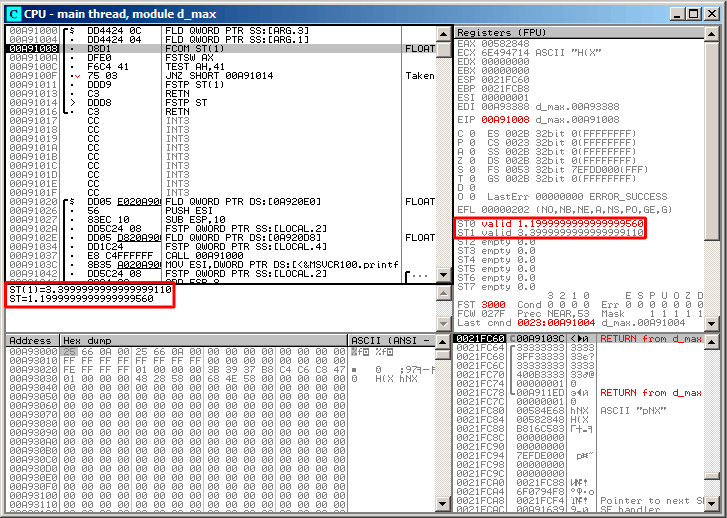
\includegraphics[scale=\FigScale]{patterns/12_FPU/3_comparison/x86/MSVC_Ox/olly1_1.png}
\caption{\olly: \RU{обе \FLD исполнились}\EN{both \FLD executed}}
\label{fig:FPU_comparison_Ox_case1_olly1}
\end{figure}

\begin{figure}[H]
\centering
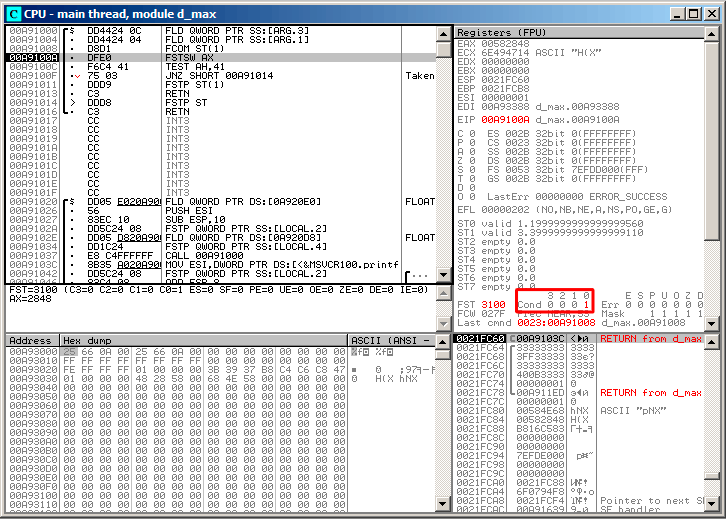
\includegraphics[scale=\FigScale]{patterns/12_FPU/3_comparison/x86/MSVC_Ox/olly1_2.png}
\caption{\olly: \FCOM \RU{исполнилась}\EN{executed}}
\label{fig:FPU_comparison_Ox_case1_olly2}
\end{figure}

\begin{figure}[H]
\centering
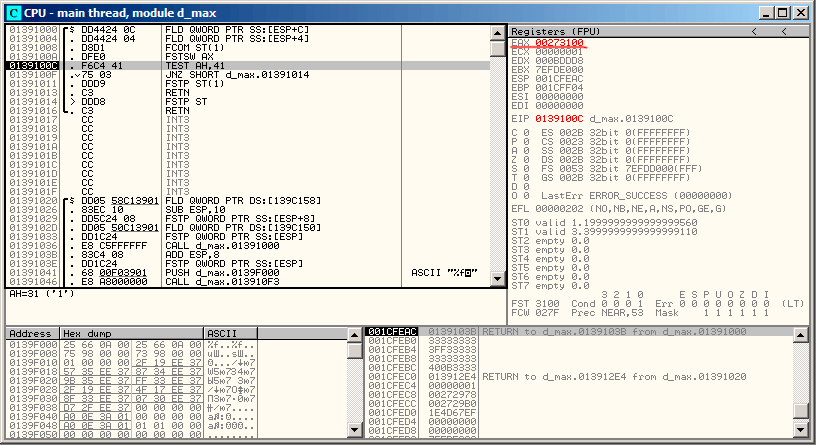
\includegraphics[scale=\FigScale]{patterns/12_FPU/3_comparison/x86/MSVC_Ox/olly1_3.png}
\caption{\olly: \FNSTSW \RU{исполнилась}\EN{executed}}
\label{fig:FPU_comparison_Ox_case1_olly3}
\end{figure}

\begin{figure}[H]
\centering
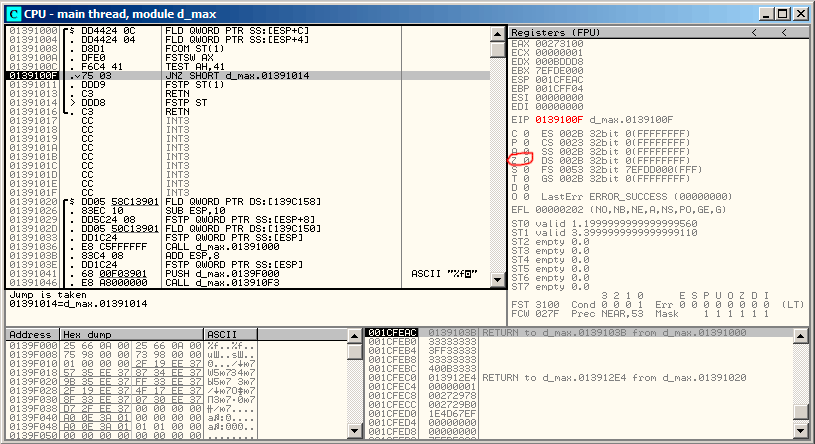
\includegraphics[scale=\FigScale]{patterns/12_FPU/3_comparison/x86/MSVC_Ox/olly1_4.png}
\caption{\olly: \TEST \RU{исполнилась}\EN{executed}}
\label{fig:FPU_comparison_Ox_case1_olly4}
\end{figure}

\begin{figure}[H]
\centering
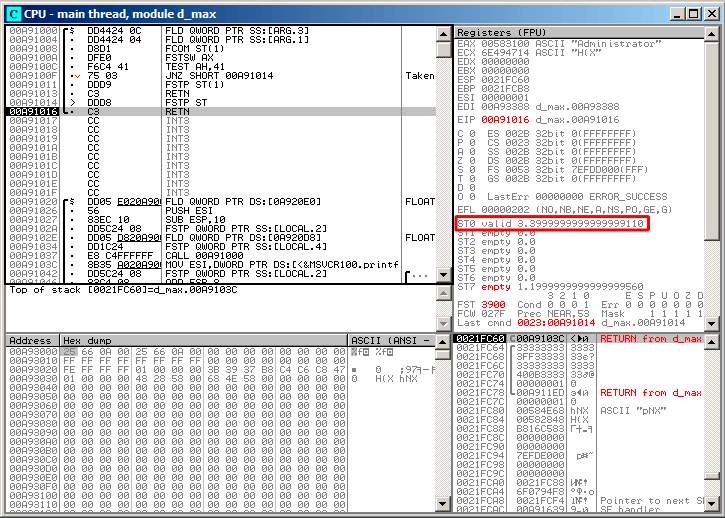
\includegraphics[scale=\FigScale]{patterns/12_FPU/3_comparison/x86/MSVC_Ox/olly1_5.png}
\caption{\olly: \FSTP \RU{исполнилась}\EN{executed}}
\label{fig:FPU_comparison_Ox_case1_olly5}
\end{figure}

\myparagraph{\RU{Второй пример с \olly}\EN{Second \olly example}: a=5.6 \AndENRU b=-4}

\RU{Обе}\EN{Both} \FLD \RU{отработали}\EN{executed}: \figref{fig:FPU_comparison_Ox_case2_olly1}.
\RU{Сейчас будет исполняться }\FCOMP\EN{ being executed}.

\FCOM \RU{сработала}\EN{done}: \figref{fig:FPU_comparison_Ox_case2_olly2}.
\RU{Все condition-флаги сброшены}\EN{All condition-flags are cleared}.

\FNSTSW \RU{сработала}\EN{done}, \TT{AX}=0x3000: \figref{fig:FPU_comparison_Ox_case2_olly3}.

\TEST \RU{сработала}\EN{is done}: \figref{fig:FPU_comparison_Ox_case2_olly4}.
ZF=1, \RU{переход сейчас не произойдет}\EN{jump will not be triggered now}.

\FSTP \ST{1} \RU{сработала: на вершине FPU-стека осталось значение $5.6$}\EN{was executed: a value
of $5.6$ is now at the top of FPU-stack}.
\figref{fig:FPU_comparison_Ox_case2_olly5}.
\RU{Видно, что инструкция}\EN{We now see that} \FSTP \ST{1} 
\RU{работает так: оставляет значение на вершине стека, но обнуляет регистр \ST{1}}
\EN{instruction works as follows: it leaves what was at the top of stack, but clears \ST{1} register}.

\begin{figure}[H]
\centering
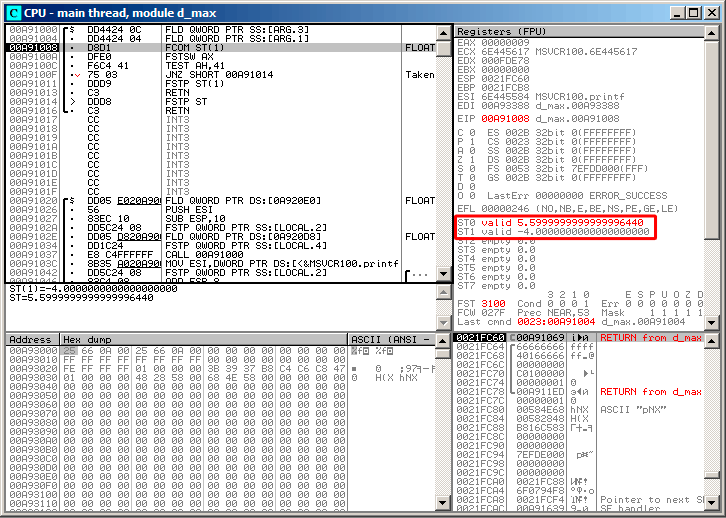
\includegraphics[scale=\FigScale]{patterns/12_FPU/3_comparison/x86/MSVC_Ox/olly2_1.png}
\caption{\olly: \RU{обе \FLD исполнились}\EN{both \FLD executed}}
\label{fig:FPU_comparison_Ox_case2_olly1}
\end{figure}

\begin{figure}[H]
\centering
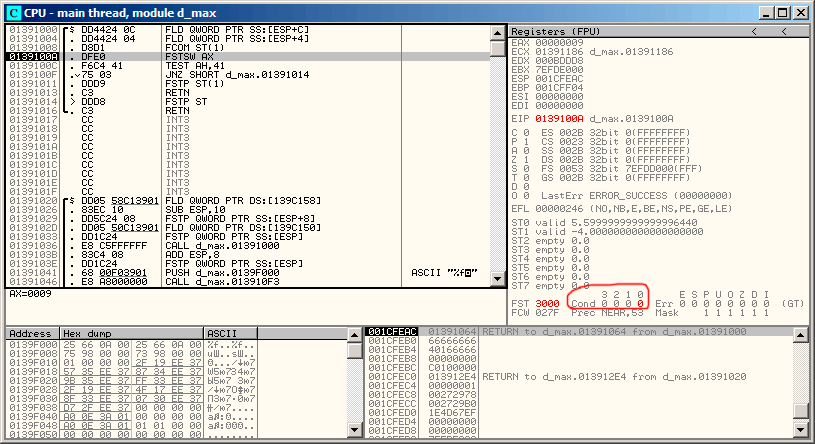
\includegraphics[scale=\FigScale]{patterns/12_FPU/3_comparison/x86/MSVC_Ox/olly2_2.png}
\caption{\olly: \FCOM \RU{исполнилась}\EN{executed}}
\label{fig:FPU_comparison_Ox_case2_olly2}
\end{figure}

\begin{figure}[H]
\centering
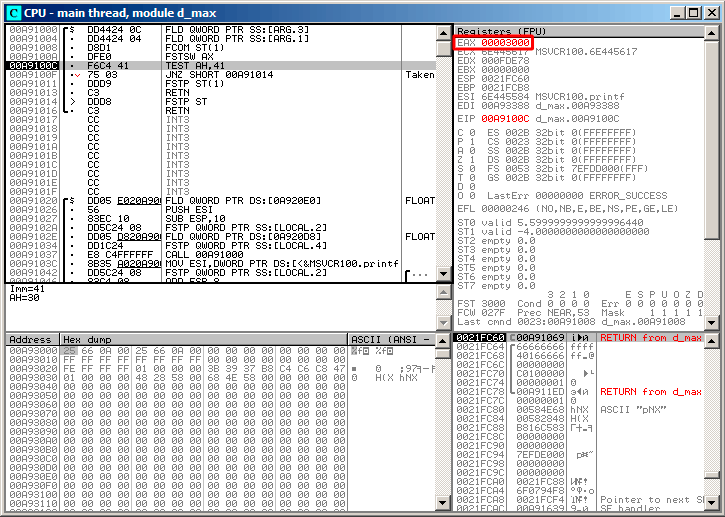
\includegraphics[scale=\FigScale]{patterns/12_FPU/3_comparison/x86/MSVC_Ox/olly2_3.png}
\caption{\olly: \FNSTSW \RU{исполнилась}\EN{executed}}
\label{fig:FPU_comparison_Ox_case2_olly3}
\end{figure}

\begin{figure}[H]
\centering
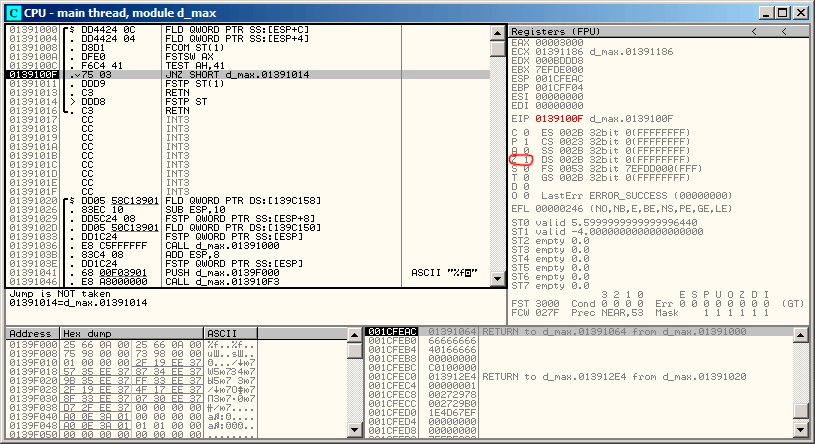
\includegraphics[scale=\FigScale]{patterns/12_FPU/3_comparison/x86/MSVC_Ox/olly2_4.png}
\caption{\olly: \TEST \RU{исполнилась}\EN{executed}}
\label{fig:FPU_comparison_Ox_case2_olly4}
\end{figure}

\begin{figure}[H]
\centering
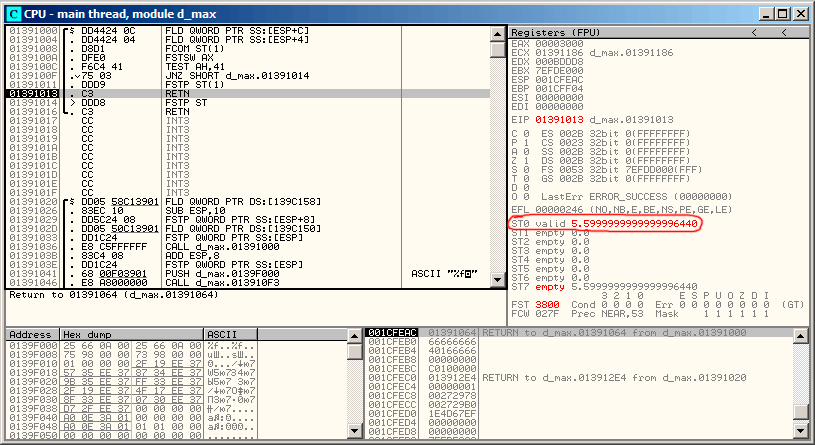
\includegraphics[scale=\FigScale]{patterns/12_FPU/3_comparison/x86/MSVC_Ox/olly2_5.png}
\caption{\olly: \FSTP \RU{исполнилась}\EN{executed}}
\label{fig:FPU_comparison_Ox_case2_olly5}
\end{figure}

\subsubsection{GCC 4.4.1}

\lstinputlisting[caption=GCC 4.4.1]{patterns/12_FPU/3_comparison/x86/GCC_\LANG.asm}

\index{x86!\Instructions!FUCOMPP}
\RU{\FUCOMPP ~--- это почти то же что и \FCOM, только выкидывает из стека оба значения после сравнения, 
а также несколько иначе реагирует на ``не-числа''.}
\EN{\FUCOMPP{}~---is almost like \FCOM, but popping both values from stack and handling 
``not-a-numbers'' differently.}

\index{\RU{Не-числа}\EN{Non-a-numbers} (NaNs)}
\RU{Немного о \IT{не-числах}}\EN{More about \IT{not-a-numbers}}:

\newcommand{\NANFN}{\RU{\footnote{\url{http://ru.wikipedia.org/wiki/NaN}}}
\EN{\footnote{\url{http://en.wikipedia.org/wiki/NaN}}}}

\RU{FPU умеет работать со специальными переменными, которые числами не являются и называются ``не числа'' или 
\gls{NaN}\NANFN{}. 
Это бесконечность, результат деления на ноль, и так далее. Нечисла бывают ``тихие'' и ``сигнализирующие''. 
С первыми можно продолжать работать и далее, а вот если вы попытаетесь совершить какую-то операцию 
с сигнализирующим нечислом, то сработает исключение.}
\EN{FPU is able to deal with a special values which are \IT{not-a-numbers} or 
\gls{NaN}s\NANFN{}. 
These are infinity, result of dividing by $0$, etc. 
Not-a-numbers can be ``quiet'' and ``signaling''. It is possible to continue to work with ``quiet'' NaNs, 
but if one try to do any operation with ``signaling'' NaNs~---an exception will be raised.}

\index{x86!\Instructions!FCOM}
\index{x86!\Instructions!FUCOM}
\RU{Так вот, \FCOM вызовет исключение если любой из операндов ~--- какое-либо нечисло.
\FUCOM же вызовет исключение только если один из операндов именно ``сигнализирующее нечисло''.}
\EN{\FCOM will raise exception if any operand~---\gls{NaN}. 
\FUCOM will raise exception only if any operand~---signaling \gls{NaN} (SNaN).}

\index{x86!\Instructions!SAHF}
\label{SAHF}
\RU{Далее мы видим \SAHF ~--- это довольно редкая инструкция в коде не использующим FPU. 
8 бит из \AH перекладываются в младшие 8 бит регистра статуса процессора в таком порядке: 
\TT{SF:ZF:-:AF:-:PF:-:CF <- AH}.}
\EN{The following instruction is \SAHF~---this is rare instruction in the code which is not use FPU. 
8 bits from AH is movinto into lower 8 bits of CPU flags in the following order: 
\TT{SF:ZF:-:AF:-:PF:-:CF <- AH}.}

\index{x86!\Instructions!FNSTSW}
\RU{Вспомним, что \FNSTSW перегружает интересующие нас биты \CThreeBits в \AH, 
и соответственно они будут в позициях 6, 2, 0 в регистре \AH.}
\EN{Let's remember the \FNSTSW is moving interesting for us bits \CThreeBits into the \AH 
and they will be in positions 6, 2, 0 in the \AH register.}

\RU{Иными словами, пара инструкций \TT{fnstsw  ax / sahf} перекладывает биты \CThreeBits в флаги \ZF, \PF, \CF.}
\EN{In other words, \TT{fnstsw  ax / sahf} instruction pair is moving \CThreeBits into \ZF, \PF, \CF CPU flags.}

\RU{Теперь снова вспомним, какие значения бит \CThreeBits будут при каких результатах сравнения:}
\EN{Now let's also recall, what values of the \CThreeBits bits will be set:}

\begin{itemize}
\item
\RU{Если a больше b в нашем случае, то биты \CThreeBits должны быть выставлены так:}
\EN{If a is greater than b in our example, then \CThreeBits bits will be set as:} 0, 0, 0.
\item
\RU{Если a меньше b, то биты будут выставлены:}\EN{if a is less than b, then bits will be set as:} 0, 0, 1.
\item
\RU{Если a=b, то биты будут выставлены так:}\EN{If a=b, then bits will be set:} 1, 0, 0.
\end{itemize}
% TODO: table?

\RU{Иными словами, после инструкций \FUCOMPP/\FNSTSW/\SAHF, мы получим такое состояние флагов:}
\EN{In other words, after \FUCOMPP/\FNSTSW/\SAHF instructions, we will have these CPU flags states:}

\begin{itemize}
\item
\RU{Если a>b в нашем случае, то флаги будут выставлены так:}
\EN{If a>b, CPU flags will be set as:} \TT{ZF=0, PF=0, CF=0}.
\item
\RU{Если a<b, то флаги будут выставлены:}\EN{If a<b, then CPU flags will be set as:} \TT{ZF=0, PF=0, CF=1}.
\item
\RU{Если a=b, то флаги будут выставлены так:}\EN{If a=b, then CPU flags will be set as:} \TT{ZF=1, PF=0, CF=0}.
\end{itemize}
% TODO: table?

\index{x86!\Instructions!SETNBE}
\index{x86!\Instructions!SETcc}
\index{x86!\Instructions!JNBE}
\RU{Инструкция \SETNBE выставит в \AL единицу или ноль, в зависимости от флагов и условий. 
Это почти аналог \JNBE, за тем лишь исключением, что \SETcc
\footnote{\IT{cc} это \IT{condition code}}
выставляет 1 или 0 в \AL, а \Jcc делает переход или нет. 
\SETNBE запишет 1 если только \TT{CF=0} и \TT{ZF=0}. Если это не так, то запишет $0$ в \AL.}
\EN{How \SETNBE instruction will store 1 or 0 to AL: it is depends of CPU flags. 
It is almost \JNBE instruction counterpart, with the exception the \SETcc 
\footnote{\IT{cc} is \IT{condition code}} is storing 1 or 0 to the \AL, but \Jcc do actual jump or not. 
\SETNBE store 1 only if \TT{CF=0} and \TT{ZF=0}. If it is not true, $0$ will be stored into \AL.}

\RU{\CF будет 0 и \ZF будет 0 одновременно только в одном случае: если a>b.}
\EN{Both \CF is 0 and \ZF is 0 simultaneously only in one case: if a>b.}

\RU{Тогда в \AL будет записана единица, последующий условный переход \JZ взят не будет, 
и функция вернет \TT{\_a}. 
В остальных случаях, функция вернет \TT{\_b}.}
\EN{Then one will be stored to the \AL and the following \JZ will not be triggered and function will 
return {\_a}. In all other cases, {\_b} will be returned.}


\subsubsection{\Optimizing GCC 4.4.1}

\lstinputlisting[caption=\Optimizing GCC 4.4.1]{patterns/12_FPU/3_comparison/x86/GCC_O3.asm.\LANG}

\index{x86!\Instructions!JA}

\ifdefined\ENGLISH
It is almost the same except that \JA is used after \SAHF. 
Actually, conditional jump instructions that check \q{larger}, \q{lesser} or \q{equal} for unsigned number comparison 
(these are \JA, \JAE, \JB, \JBE, \JE/\JZ, \JNA, \JNAE, \JNB, \JNBE, \JNE/\JNZ) check only flags \CF and \ZF.\\
\\
Let's recall where bits \CThreeBits are located in the \TT{AH} register after the execution of \TT{FSTSW}/\FNSTSW:

\input{C3_in_AH}

Let's also recall, how the bits from \TT{AH} are stored into the CPU flags the execution of \SAHF:

\input{SAHF_LAHF}

After the comparison, the \Cthree and \Czero bits are moved into \ZF and \CF, so the conditional jumps are able work after. \JA is triggering if both \CF are \ZF zero.

Thereby, the conditional jumps instructions listed here can be used after a \FNSTSW/\SAHF instruction pair.

Apparently, the FPU \CThreeBits status bits were placed there intentionally, to easily map them to base CPU flags without additional permutations?
\fi % ENGLISH

\ifdefined\RUSSIAN
Почти всё что здесь есть, уже описано мною, кроме одного: использование \JA после \SAHF. 
Действительно, инструкции условных переходов \q{больше}, \q{меньше} и \q{равно} для сравнения беззнаковых чисел 
(а это \JA, \JAE, \JB, \JBE, \JE/\JZ, \JNA, \JNAE, \JNB, \JNBE, \JNE/\JNZ) проверяют только флаги \CF и \ZF.\\
\\
Вспомним, как биты \CThreeBits располагаются в регистре \TT{AH} после исполнения \TT{FSTSW}/\FNSTSW:

\input{C3_in_AH}

Вспомним также, как располагаются биты из \TT{AH} во флагах CPU после исполнения \SAHF:

\input{SAHF_LAHF}

Биты \Cthree и \Czero после сравнения перекладываются в флаги \ZF и \CF так, что перечисленные инструкции переходов могут работать. \JA сработает, если \CF и \ZF обнулены.

Таким образом, перечисленные инструкции условного перехода можно использовать после инструкций \FNSTSW/\SAHF.

Может быть, биты статуса FPU \CThreeBits преднамеренно были размещены таким образом, чтобы переноситься на базовые флаги процессора без перестановок?
\fi % RUSSIAN


\subsubsection{GCC 4.8.1 \RU{с оптимизацией \Othree}\EN{with \Othree optimization turned on}}

\EN{Some new FPU instructions were appeared in P6 Intel family}\RU{В линейке процессоров P6 от Intel 
появились новые FPU-инструкции}\footnote{\EN{Starting at}\RU{Начиная с} Pentium Pro, 
Pentium-II, \RU{итд}\EN{etc}}.
\RU{Это}\EN{These are} \TT{FUCOMI} (\RU{сравнить операнды и выставить флаги основного CPU}\EN{compare 
operands and set flags of main CPU}) \AndENRU 
\TT{FCMOVcc} (\RU{работает как}\EN{works like} \TT{CMOVcc}, \RU{но на регистрах FPU}\EN{but on FPU registers}).
\RU{Очевидно, разработчики GCC решили отказаться от поддержки процессоров до линейки P6 (ранние Pentium, итд)}
\EN{Apparently, GCC maintainers decided to drop support of Intel CPUs before P6 family (early Pentiums, etc)}.

\RU{И похоже, FPU уже давно не отдельная часть процессора в линейке P6, так что флаги основного CPU можно
модифицировать из FPU.}
\EN{It seems, FPU is no longer separate unit in P6 Intel family, so now it is possible to modify/check flags 
of main CPU from FPU.}

\RU{Вот что имеем}\EN{So what we got is}:

\lstinputlisting[caption=\Optimizing GCC 4.8.1]{patterns/12_FPU/3_comparison/x86/GCC481_O3.s}

\RU{Не совсем понимаю, зачем здесь \TT{FXCH} (поменять местами операнды)}
\EN{I'm not sure why \TT{FXCH} (swap operands) is here}.
\RU{От нее легко избавиться поменяв местами инструкции \FLD либо заменив 
\TT{FCMOVBE} (\IT{below or equal} --- меньше или равно) на 
\TT{FCMOVA} (\IT{above} --- больше).}
\EN{It's possible to get rid of it easily by swapping two first \FLD instructions or by replacing 
\TT{FCMOVBE} (\IT{below or equal}) by \TT{FCMOVA} (\IT{above}).}
\RU{Должно быть, неаккуратность компилятора}\EN{Probably, compiler's inaccuracy}.

\RU{Так что}\EN{So} \TT{FUCOMI} \EN{compares}\RU{сравниванет} \ST{0} ($a$) \AndENRU \ST{1} ($b$) 
\RU{и затем устанавливает флаги основного CPU}\EN{and then sets main CPU flags}.
\TT{FCMOVBE} \RU{проверяет флаги и копирует}\EN{checks flags and copying} \ST{1} 
(\RU{в тот момент там находится $b$}\EN{$b$ here at the moment}) \RU{в}\EN{to} 
\ST{0} (\RU{там $a$}\EN{$a$ here}) \RU{если}\EN{if} $ST0 (a) <= ST1 (b)$.
\RU{В противном случае}\EN{Otherwise} ($a>b$), \RU{она оставляет}\EN{it leaves} $a$ \InENRU \ST{0}.

\RU{Последняя}\EN{The last} \FSTP \RU{оставляет содержимое}\EN{leaves} \ST{0} 
\RU{на вершине стека, выбрасывая содержимое}\EN{on top of stack discarding} \ST{1}\EN{ contents}.

\RU{Попробуем оттрасировать ф-цию в}\EN{Let's trace this function in} GDB:

\lstinputlisting[caption=\Optimizing GCC 4.8.1 and GDB,numbers=left]{patterns/12_FPU/3_comparison/x86/gdb.txt}

\RU{Используя}\EN{Using} ``ni'', \RU{дадим первым двум инструкциям \FLD исполниться.}
\EN{let's execute two first \FLD instructions.}

\RU{Посмотрим регистры FPU}\EN{Let's examine FPU registers} (\LineENRU 33).

\RU{Как я писал раннее, регистры FPU это скорее кольцевой буфер, нежели стек}
\EN{As I wrote before, FPU registers are circular buffer rather than stack} (\ref{FPU_is_rather_circular_buffer}).
\RU{И}\EN{And} GDB \RU{показывает не регистры}\EN{shows not} \TT{STx} \RU{а внутренние регистры FPU}
\EN{registers, but internal FPU registers} (\TT{Rx}). 
\RU{Стрелка}\EN{Arrow} (\RU{на строке}\EN{at line} 35) 
\RU{указывает на текущую вершину стека.}
\EN{points to the current stack top.}
\RU{Вы можете также увидеть переменную \TT{TOP} в ``Status Word'' (строка 44), там сейчас 6, так что
вершина стека это сейчас внутренний регистр 6.}
\EN{You may also see \TT{TOP} variable in \IT{Status Word} (line 44) it has 6 now, 
so stack top is now in internal register 6.}

\RU{Значения $a$ и $b$ меняются местами после исполнения \TT{FXCH}}\EN{$a$ and $b$ values are swapped 
after \TT{FXCH} executed} (\LineENRU 54).

\TT{FUCOMI} \RU{исполнилась}\EN{executed} (\LineENRU 83). 
\RU{Посмотрим флаги}\EN{Let's see flags}: \CF \RU{выставлен}\EN{is set} (\LineENRU 95).

\TT{FCMOVBE} \RU{действительно скопировал значение $b$ (см.строку 104).}
\EN{is actually copied value of $b$ (see line 104).}

\FSTP \RU{оставляет одно значение на вершине стека}\EN{leaves one value at the top of stack} (\LineENRU 136). 
\RU{Значение \TT{TOP} теперь 7, так что вершина FPU-стека указывает на внутренний регистр 7}\EN{\TT{TOP} value is 
now 7, so FPU stack top is points to internal register 7}.

% TODO task: rewrite the function without FXCH and test it



\EN{\subsubsection{ARM}

\myparagraph{\OptimizingXcodeIV (\ARMMode)}

\lstinputlisting[caption=\OptimizingXcodeIV (\ARMMode)]{patterns/12_FPU/3_comparison/ARM/Xcode_ARM_EN.lst}

\myindex{ARM!\Registers!APSR}
\myindex{ARM!\Registers!FPSCR}
A very simple case.
The input values are placed into the \GTT{D17} and \GTT{D16} registers and then compared using the \INS{VCMPE} instruction.

Just like in the x86 coprocessor, the ARM coprocessor has its own status and flags register (\ac{FPSCR}),
since there is a need to store coprocessor-specific flags.
% TODO -> расписать регистр по битам
\myindex{ARM!\Instructions!VMRS}
And just like in x86, there are no conditional jump instruction in ARM, 
that can check bits in the status register of the coprocessor. 
So there is \INS{VMRS}, which copies 4 bits (N, Z, C, V) from the coprocessor status word into bits of the \IT{general} status register (\ac{APSR}).

\myindex{ARM!\Instructions!VMOVGT}
\INS{VMOVGT} is the analog of the \INS{MOVGT}, 
instruction for D-registers, it executes if one operand is greater than the other while comparing (\IT{GT---Greater Than}). 

If it gets executed, the value of $b$ is to be written into \GTT{D16} (that is currently stored in in \GTT{D17}).
Otherwise the value of $a$ stays in the \GTT{D16} register.

\myindex{ARM!\Instructions!VMOV}

The penultimate instruction \INS{VMOV} prepares the value in the \GTT{D16} register for returning it via the \Reg{0} and \Reg{1}
register pair.

\myparagraph{\OptimizingXcodeIV (\ThumbTwoMode)}

\begin{lstlisting}[caption=\OptimizingXcodeIV (\ThumbTwoMode)]
VMOV            D16, R2, R3 ; b
VMOV            D17, R0, R1 ; a
VCMPE.F64       D17, D16
VMRS            APSR_nzcv, FPSCR
IT GT 
VMOVGT.F64      D16, D17
VMOV            R0, R1, D16
BX              LR
\end{lstlisting}

Almost the same as in the previous example, however slightly different.
As we already know, many instructions in ARM mode can be supplemented by condition predicate.
But there is no such thing in Thumb mode. 
There is no space in the 16-bit instructions for 4 more bits in which conditions can be encoded.

\myindex{ARM!\ThumbTwoMode}

However, Thumb-2 was extended to make it possible to specify predicates to old Thumb instructions.
Here, in the \IDA-generated listing, we see the \INS{VMOVGT} instruction, as in previous example.

In fact, the usual \INS{VMOV} is encoded there, but \IDA adds the \GTT{-GT} suffix to it, 
since there is a \INS{IT GT} instruction placed right before it.

\label{ARM_Thumb_IT}
\myindex{ARM!\Instructions!IT}
\myindex{ARM!if-then block}
The \INS{IT} instruction defines a so-called \IT{if-then block}. 

After the instruction it is possible to place up to 4 instructions, 
each of them has a predicate suffix.
In our example, \INS{IT GT} implies that the next instruction is to be executed, if the \IT{GT} (\IT{Greater Than}) condition is true.

\myindex{Angry Birds}
Here is a more complex code fragment, by the way, from Angry Birds (for iOS):

\begin{lstlisting}[caption=Angry Birds Classic]
...
ITE NE
VMOVNE          R2, R3, D16
VMOVEQ          R2, R3, D17
BLX             _objc_msgSend ; not suffixed
...
\end{lstlisting}

\INS{ITE} stands for \IT{if-then-else} 

and it encodes suffixes for the next two instructions.

The first instruction executes if the condition encoded in \INS{ITE} (\IT{NE, not equal}) is true at, and the second---if the condition is not true.
(The inverse condition of \GTT{NE} is \GTT{EQ} (\IT{equal})).

The instruction followed after the second \INS{VMOV} (or \INS{VMOVEQ}) is a normal one, not suffixed (\INS{BLX}).

\myindex{Angry Birds}
One more that's slightly harder, which is also from Angry Birds:

\begin{lstlisting}[caption=Angry Birds Classic]
...
ITTTT EQ
MOVEQ           R0, R4
ADDEQ           SP, SP, #0x20
POPEQ.W         {R8,R10}
POPEQ           {R4-R7,PC}
BLX             ___stack_chk_fail ; not suffixed
...
\end{lstlisting}

Four \q{T} symbols in the instruction mnemonic mean that the four subsequent instructions are to be executed if the condition is true.

That's why \IDA adds the \GTT{-EQ} suffix to each one of them. 

And if there was be, for example, \INS{ITEEE EQ} (\IT{if-then-else-else-else}), 

then the suffixes would have been set as follows:

\begin{lstlisting}
-EQ
-NE
-NE
-NE
\end{lstlisting}

\myindex{Angry Birds}
Another fragment from Angry Birds:

\begin{lstlisting}[caption=Angry Birds Classic]
...
CMP.W           R0, #0xFFFFFFFF
ITTE LE
SUBLE.W         R10, R0, #1
NEGLE           R0, R0
MOVGT           R10, R0
MOVS            R6, #0         ; not suffixed
CBZ             R0, loc_1E7E32 ; not suffixed
...
\end{lstlisting}

\INS{ITTE} (\IT{if-then-then-else}) 

implies that the 1st and 2nd instructions are to be executed if the \GTT{LE} (\IT{Less or Equal})
condition is true, and the 3rd---if the inverse condition (\GTT{GT}\EMDASH\IT{Greater Than}) 
is true.

Compilers usually don't generate all possible combinations.
\myindex{Angry Birds}

For example, in the mentioned Angry Birds game (\IT{classic} version for iOS)
only these variants of the \INS{IT} instruction are used: 
\INS{IT}, \INS{ITE}, \INS{ITT}, \INS{ITTE}, \INS{ITTT}, \INS{ITTTT}.
\myindex{\GrepUsage}
How to learn this?
In \IDA It is possible to produce listing files, so it was created with an option to show 4 bytes for each opcode.
Then, knowing the high part of the 16-bit opcode (\INS{IT} is \GTT{0xBF}), we do the following using \GTT{grep}:

\begin{lstlisting}
cat AngryBirdsClassic.lst | grep " BF" | grep "IT" > results.lst
\end{lstlisting}

\myindex{ARM!\ThumbTwoMode}

By the way, if you program in ARM assembly language manually for Thumb-2 mode, 
and you add conditional suffixes,
the assembler will add the \INS{IT} instructions automatically with the required flags where it is necessary.

\myparagraph{\NonOptimizingXcodeIV (\ARMMode)}

\begin{lstlisting}[caption=\NonOptimizingXcodeIV (\ARMMode)]
b               = -0x20
a               = -0x18
val_to_return   = -0x10
saved_R7        = -4

                STR             R7, [SP,#saved_R7]!
                MOV             R7, SP
                SUB             SP, SP, #0x1C
                BIC             SP, SP, #7
                VMOV            D16, R2, R3
                VMOV            D17, R0, R1
                VSTR            D17, [SP,#0x20+a]
                VSTR            D16, [SP,#0x20+b]
                VLDR            D16, [SP,#0x20+a]
                VLDR            D17, [SP,#0x20+b]
                VCMPE.F64       D16, D17
                VMRS            APSR_nzcv, FPSCR
                BLE             loc_2E08
                VLDR            D16, [SP,#0x20+a]
                VSTR            D16, [SP,#0x20+val_to_return]
                B               loc_2E10

loc_2E08
                VLDR            D16, [SP,#0x20+b]
                VSTR            D16, [SP,#0x20+val_to_return]

loc_2E10
                VLDR            D16, [SP,#0x20+val_to_return]
                VMOV            R0, R1, D16
                MOV             SP, R7
                LDR             R7, [SP+0x20+b],#4
                BX              LR
\end{lstlisting}

Almost the same as we already saw, 
but there is too much redundant code because the $a$ and $b$ variables are stored in the local stack, as well
as the return value.

\myparagraph{\OptimizingKeilVI (\ThumbMode)}

\begin{lstlisting}[caption=\OptimizingKeilVI (\ThumbMode)]
                PUSH    {R3-R7,LR}
                MOVS    R4, R2
                MOVS    R5, R3
                MOVS    R6, R0
                MOVS    R7, R1
                BL      __aeabi_cdrcmple
                BCS     loc_1C0
                MOVS    R0, R6
                MOVS    R1, R7
                POP     {R3-R7,PC}

loc_1C0
                MOVS    R0, R4
                MOVS    R1, R5
                POP     {R3-R7,PC}
\end{lstlisting}


Keil doesn't generate FPU-instructions since it cannot rely on them being
supported on the target CPU, and it cannot be done by straightforward bitwise comparing.
%TODO1: why?
So it calls an external library function to do the comparison: \GTT{\_\_aeabi\_cdrcmple}. 
\myindex{ARM!\Instructions!BCS}

N.B. The result of the comparison is to be left in the flags by this function, so the following
\INS{BCS} (\IT{Carry set---Greater than or equal})
instruction can work without any additional code.

}
\RU{\subsectionold{ARM}

\subsubsectionold{\OptimizingXcodeIV (\ARMMode)}

\lstinputlisting[caption=\OptimizingXcodeIV (\ARMMode)]{patterns/12_FPU/3_comparison/ARM/Xcode_ARM_RU.lst}

\myindex{ARM!\Registers!APSR}
\myindex{ARM!\Registers!FPSCR}
Очень простой случай.
Входные величины помещаются в \GTT{D17} и \GTT{D16} и сравниваются при помощи инструкции \INS{VCMPE}.
Как и в сопроцессорах x86, сопроцессор в ARM имеет свой собственный регистр статуса и флагов (\ac{FPSCR}),
потому что есть необходимость хранить специфичные для его работы флаги.

% TODO -> расписать регистр по битам
\myindex{ARM!\Instructions!VMRS}
И так же, как и в x86, 
в ARM нет инструкций условного перехода, проверяющих биты в регистре статуса сопроцессора. 
Поэтому имеется инструкция \INS{VMRS}, копирующая 4 бита (N, Z, C, V) 
из статуса сопроцессора в биты \IT{общего} статуса (регистр \ac{APSR}).

\myindex{ARM!\Instructions!VMOVGT}
\INS{VMOVGT} это аналог \INS{MOVGT}, инструкция для D-регистров, срабатывающая, если при сравнении один операнд был больше чем второй
(\IT{GT\EMDASH{}Greater Than}). 

Если она сработает, 
в \GTT{D16} запишется значение $b$, лежащее в тот момент в \GTT{D17}.
В обратном случае в \GTT{D16} остается значение $a$.


\myindex{ARM!\Instructions!VMOV}
Предпоследняя инструкция \INS{VMOV} готовит то, что было в \GTT{D16}, для возврата через 
пару регистров \Reg{0} и \Reg{1}.

\subsubsectionold{\OptimizingXcodeIV (\ThumbTwoMode)}

\begin{lstlisting}[caption=\OptimizingXcodeIV (\ThumbTwoMode)]
VMOV            D16, R2, R3 ; b
VMOV            D17, R0, R1 ; a
VCMPE.F64       D17, D16
VMRS            APSR_nzcv, FPSCR
IT GT 
VMOVGT.F64      D16, D17
VMOV            R0, R1, D16
BX              LR
\end{lstlisting}

Почти то же самое, что и в предыдущем примере, за парой отличий.
Как мы уже знаем, многие инструкции в режиме ARM можно дополнять условием.
Но в режиме Thumb такого нет.
В 16-битных инструкций просто нет места для лишних 4 битов, при помощи
которых можно было бы закодировать условие выполнения.

\myindex{ARM!\ThumbTwoMode}
Поэтому в Thumb-2 добавили возможность дополнять Thumb-инструкции условиями.
В листинге, сгенерированном при помощи \IDA, мы видим инструкцию \INS{VMOVGT}, 
такую же как и в предыдущем примере.

В реальности там закодирована обычная инструкция \INS{VMOV}, просто \IDA добавила суффикс \GTT{-GT} к ней, 
потому что перед этой инструкцией стоит \INS{IT GT}.

\label{ARM_Thumb_IT}
\myindex{ARM!\Instructions!IT}
\myindex{ARM!if-then block}
Инструкция \INS{IT} определяет так называемый \IT{if-then block}. 
После этой инструкции можно указывать до четырех инструкций, 
к каждой из которых будет добавлен суффикс условия.

В нашем примере \INS{IT GT} означает,
что следующая за ней инструкция будет исполнена, если условие
\IT{GT} (\IT{Greater Than}) справедливо.

\myindex{Angry Birds}
Теперь более сложный пример. Кстати, из 
Angry Birds (для iOS):

\begin{lstlisting}[caption=Angry Birds Classic]
...
ITE NE
VMOVNE          R2, R3, D16
VMOVEQ          R2, R3, D17
BLX             _objc_msgSend ; без суффикса
...
\end{lstlisting}

\INS{ITE} означает \IT{if-then-else} 
и кодирует суффиксы для двух следующих за ней инструкций.

Первая из них исполнится, если условие, закодированное в \INS{ITE} (\IT{NE, not equal}) будет в тот момент справедливо,
а вторая~--- если это условие не сработает.
(Обратное условие от \GTT{NE} это \GTT{EQ} (\IT{equal})).

Инструкция следующая за второй \INS{VMOV} (или VMOEQ) нормальная, без суффикса (\INS{BLX}).

\myindex{Angry Birds}
Ещё чуть сложнее, и снова этот фрагмент из Angry Birds:

\begin{lstlisting}[caption=Angry Birds Classic]
...
ITTTT EQ
MOVEQ           R0, R4
ADDEQ           SP, SP, #0x20
POPEQ.W         {R8,R10}
POPEQ           {R4-R7,PC}
BLX             ___stack_chk_fail ; без суффикса
...
\end{lstlisting}

Четыре символа \q{T} в инструкции означают, что четыре последующие инструкции будут исполнены если условие соблюдается.
Поэтому \IDA добавила ко всем четырем инструкциям суффикс \GTT{-EQ}. 
А если бы здесь было, например,
\INS{ITEEE EQ} (\IT{if-then-else-else-else}), 
тогда суффиксы для следующих четырех инструкций были бы расставлены так:

\begin{lstlisting}
-EQ
-NE
-NE
-NE
\end{lstlisting}

\myindex{Angry Birds}
Ещё фрагмент из Angry Birds:

\begin{lstlisting}[caption=Angry Birds Classic]
...
CMP.W           R0, #0xFFFFFFFF
ITTE LE
SUBLE.W         R10, R0, #1
NEGLE           R0, R0
MOVGT           R10, R0
MOVS            R6, #0         ; без суффикса
CBZ             R0, loc_1E7E32 ; без суффикса
...
\end{lstlisting}

\INS{ITTE} (\IT{if-then-then-else}) 
означает, что первая и вторая инструкции исполнятся, если условие \GTT{LE} (\IT{Less or Equal})
справедливо, а третья~--- если справедливо обратное условие (\GTT{GT}\EMDASH\IT{Greater Than}).

Компиляторы способны генерировать далеко не все варианты.

\myindex{Angry Birds}
Например, в вышеупомянутой игре Angry Birds (версия \IT{classic} для iOS)

встречаются только такие варианты инструкции \INS{IT}: 
\INS{IT}, \INS{ITE}, \INS{ITT}, \INS{ITTE}, \INS{ITTT}, \INS{ITTTT}.
\myindex{\GrepUsage}
Как это узнать?
В \IDA можно сгенерировать листинг (что и было сделано), только в опциях был установлен показ 4 байтов для каждого опкода.

Затем, зная что старшая часть 16-битного опкода (\INS{IT} это \GTT{0xBF}), сделаем при помощи \GTT{grep} это:

\begin{lstlisting}
cat AngryBirdsClassic.lst | grep " BF" | grep "IT" > results.lst
\end{lstlisting}

\myindex{ARM!\ThumbTwoMode}
Кстати, если писать на ассемблере для режима Thumb-2 вручную, и дополнять инструкции суффиксами
условия, то ассемблер автоматически будет добавлять инструкцию \INS{IT} с соответствующими флагами там,
где надо.

\subsubsectionold{\NonOptimizingXcodeIV (\ARMMode)}

\begin{lstlisting}[caption=\NonOptimizingXcodeIV (\ARMMode)]
b               = -0x20
a               = -0x18
val_to_return   = -0x10
saved_R7        = -4

                STR             R7, [SP,#saved_R7]!
                MOV             R7, SP
                SUB             SP, SP, #0x1C
                BIC             SP, SP, #7
                VMOV            D16, R2, R3
                VMOV            D17, R0, R1
                VSTR            D17, [SP,#0x20+a]
                VSTR            D16, [SP,#0x20+b]
                VLDR            D16, [SP,#0x20+a]
                VLDR            D17, [SP,#0x20+b]
                VCMPE.F64       D16, D17
                VMRS            APSR_nzcv, FPSCR
                BLE             loc_2E08
                VLDR            D16, [SP,#0x20+a]
                VSTR            D16, [SP,#0x20+val_to_return]
                B               loc_2E10

loc_2E08
                VLDR            D16, [SP,#0x20+b]
                VSTR            D16, [SP,#0x20+val_to_return]

loc_2E10
                VLDR            D16, [SP,#0x20+val_to_return]
                VMOV            R0, R1, D16
                MOV             SP, R7
                LDR             R7, [SP+0x20+b],#4
                BX              LR
\end{lstlisting}

Почти то же самое, что мы уже видели, 
но много избыточного кода из-за хранения $a$ и $b$, 
а также выходного значения, в локальном стеке.


\subsubsectionold{\OptimizingKeilVI (\ThumbMode)}

\begin{lstlisting}[caption=\OptimizingKeilVI (\ThumbMode)]
                PUSH    {R3-R7,LR}
                MOVS    R4, R2
                MOVS    R5, R3
                MOVS    R6, R0
                MOVS    R7, R1
                BL      __aeabi_cdrcmple
                BCS     loc_1C0
                MOVS    R0, R6
                MOVS    R1, R7
                POP     {R3-R7,PC}

loc_1C0
                MOVS    R0, R4
                MOVS    R1, R5
                POP     {R3-R7,PC}
\end{lstlisting}

Keil не генерирует FPU-инструкции, потому что не 
рассчитывает на то, что они будет поддерживаться, а простым сравнением побитово здесь не обойтись.

%TODO1: why?
Для сравнения вызывается библиотечная функция \GTT{\_\_aeabi\_cdrcmple}. 
\myindex{ARM!\Instructions!BCS}

N.B. Результат сравнения эта функция оставляет в флагах, чтобы следующая за вызовом инструкция
\INS{BCS} (\IT{Carry set~--- Greater than or equal})
могла работать без дополнительного кода.

}
\EN{\subsubsection{ARM64}

\myparagraph{\Optimizing GCC (Linaro) 4.9}

\lstinputlisting{patterns/12_FPU/3_comparison/ARM/ARM64_GCC_O3_EN.lst}

The ARM64 \ac{ISA} has FPU-instructions 
which set \ac{APSR} the CPU flags instead of \ac{FPSCR} for convenience.
The\ac{FPU} is not a separate device here anymore (at least, logically).
\myindex{ARM!\Instructions!FCMPE}
Here we see \INS{FCMPE}. It compares the two values passed in \RegD{0} and \RegD{1} (which are the first and second arguments of the function)
and sets \ac{APSR} flags (N, Z, C, V).

\myindex{ARM!\Instructions!FCSEL}
\INS{FCSEL} (\IT{Floating Conditional Select}) copies the value of \RegD{0} or \RegD{1} into \RegD{0} depending on the condition (\GTT{GT}---Greater Than),
and again, it uses flags in \ac{APSR} register instead of \ac{FPSCR}.

This is much more convenient, compared to the instruction set in older CPUs.

If the condition is true (\GTT{GT}), then the value of \RegD{0} 
is copied into \RegD{0} (i.e., nothing happens).
If the condition is not true, the value of \RegD{1} 
is copied into \RegD{0}.

\myparagraph{\NonOptimizing GCC (Linaro) 4.9}

\lstinputlisting{patterns/12_FPU/3_comparison/ARM/ARM64_GCC_EN.lst}

Non-optimizing GCC is more verbose.

First, the function saves its input argument values in the local stack (\IT{Register Save Area}).
Then the code reloads these values into registers
\RegX{0}/\RegX{1} and finally copies them to 
\RegD{0}/\RegD{1} to be compared using \INS{FCMPE}. 
A lot of redundant code, 
but that is how non-optimizing compilers work.
\INS{FCMPE} compares the values and sets the \ac{APSR} flags.
At this moment, 
the compiler is not thinking yet about the more convenient \INS{FCSEL} instruction, so it proceed using old methods: 
using the \INS{BLE} instruction (\IT{Branch if Less than or Equal}).
In the first case ($a>b$), the value of $a$ gets loaded 
into \RegX{0}.
In the other case ($a<=b$), the value of $b$ gets loaded into 
\RegX{0}.
Finally, the value from \RegX{0} gets copied into \RegD{0}, 
because the return value needs to be in this 
register.

\mysubparagraph{\Exercise}

As an exercise, you can try optimizing this piece of code 
manually by removing redundant instructions and not introducing new ones (including \INS{FCSEL}).

\myparagraph{\Optimizing GCC (Linaro) 4.9---float}

Let's also rewrite this example to use \Tfloat instead of \Tdouble.

\begin{lstlisting}
float f_max (float a, float b)
{
	if (a>b)
		return a;

	return b;
};
\end{lstlisting}

\lstinputlisting{patterns/12_FPU/3_comparison/ARM/ARM64_GCC_O3_float_EN.lst}

It is the same code, but the S-registers are used instead of D- ones.
It's because numbers of type \Tfloat are passed in 32-bit S-registers (which are in fact the lower parts of the 64-bit D-registers).

}
\RU{\subsubsection{ARM64}

\myparagraph{\Optimizing GCC (Linaro) 4.9}

\lstinputlisting{patterns/12_FPU/3_comparison/ARM/ARM64_GCC_O3_RU.lst}

В ARM64 \ac{ISA} теперь есть FPU-инструкции, устанавливающие флаги CPU \ac{APSR} вместо \ac{FPSCR} для удобства.
\ac{FPU} больше не отдельное устройство (по крайней мере логически).
\myindex{ARM!\Instructions!FCMPE}
Это \INS{FCMPE}. Она сравнивает два значения, переданных в \RegD{0} и \RegD{1} 
(а это первый и второй аргументы функции) и выставляет флаги в \ac{APSR} (N, Z, C, V).

\myindex{ARM!\Instructions!FCSEL}
\INS{FCSEL} (\IT{Floating Conditional Select}) копирует значение \RegD{0} или
\RegD{1} в \RegD{0} в зависимости от условия 
(\GTT{GT} --- Greater Than --- больше чем),
и снова, она использует флаги в регистре \ac{APSR} вместо \ac{FPSCR}.
Это куда удобнее, если сравнивать с тем набором инструкций, что был в процессорах раньше.

Если условие верно (\GTT{GT}), тогда значение из \RegD{0} копируется в \RegD{0} (т.е. ничего не происходит).
Если условие не верно, то значение \RegD{1} копируется в \RegD{0}.

\myparagraph{\NonOptimizing GCC (Linaro) 4.9}

\lstinputlisting{patterns/12_FPU/3_comparison/ARM/ARM64_GCC_RU.lst}

Неоптимизирующий GCC более многословен.
В начале функция сохраняет значения входных аргументов в локальном стеке (\IT{Register Save Area}).
Затем код перезагружает значения в регистры
\RegX{0}/\RegX{1} и наконец копирует их в 
\RegD{0}/\RegD{1} для сравнения инструкцией \INS{FCMPE}. 
Много избыточного кода, но так работают неоптимизирующие компиляторы.
\INS{FCMPE} сравнивает значения и устанавливает флаги в \ac{APSR}.
В этот момент компилятор ещё не думает о более удобной инструкции \INS{FCSEL}, так что он работает старым 
методом: 
использует инструкцию \INS{BLE} (\IT{Branch if Less than or Equal} (переход если меньше или равно)).
В одном случае ($a>b$) значение $a$ перезагружается в \RegX{0}.
В другом случае ($a<=b$) значение $b$ загружается в \RegX{0}.
Наконец, значение из \RegX{0} копируется в \RegD{0}, 
потому что возвращаемое значение оставляется в этом регистре.

\mysubparagraph{\Exercise}

Для упражнения вы можете попробовать оптимизировать этот фрагмент кода вручную, удалив избыточные инструкции,
но не добавляя новых (включая \INS{FCSEL}).

\myparagraph{\Optimizing GCC (Linaro) 4.9\EMDASH{}float}

Перепишем пример. Теперь здесь \Tfloat вместо \Tdouble.

\begin{lstlisting}
float f_max (float a, float b)
{
	if (a>b)
		return a;

	return b;
};
\end{lstlisting}

\lstinputlisting{patterns/12_FPU/3_comparison/ARM/ARM64_GCC_O3_float_RU.lst}

Всё то же самое, только используются S-регистры вместо D-.
Так что числа типа \Tfloat передаются в 32-битных S-регистрах (а это младшие части 64-битных D-регистров).

}
\subsection{MIPS}

\index{MIPS!\Registers!FCCR}
\EN{The co-processor of the MIPS processor has a condition bit which can be set in the FPU and checked in the CPU.}
\RU{В сопроцессоре MIPS есть бит результата, который устанавливается в FPU и проверяется в CPU.}
\EN{Earlier MIPS-es have only one condition bit (called FCC0), later ones have 8 (called FCC7-FCC0).}
\RU{Ранние MIPS имели только один бит (с названием FCC0), а у поздних их 8 (с названием FCC7-FCC0).}
\RU{Этот бит (или биты) находятся в регистре с названием FCCR.}
\EN{This bit (or bits) are located in the register called FCCR.}

\lstinputlisting[caption=\Optimizing GCC 4.4.5 (IDA)]{patterns/12_FPU/3_comparison/MIPS_O3_IDA.lst.\LANG}

\index{MIPS!\Instructions!C.LT.D}
\TT{C.LT.D} \EN{compares two values}\RU{сравнивает два значения}. 
\TT{LT} \EN{is the condition}\RU{это условие} \q{Less Than}\RU{ (меньше чем)}.
\TT{D} \EN{implies values of type}\RU{означает переменные типа} \Tdouble.
\EN{Depending on the result of the comparison, the FCC0 condition bit is either set or cleared.}
\RU{В зависимости от результата сравнения, бит FCC0 устанавливается или очищается.}

\index{MIPS!\Instructions!BC1T}
\index{MIPS!\Instructions!BC1F}
\TT{BC1T} \EN{checks the FCC0 bit and jumps if the bit is set}\RU{проверяет бит FCC0 и делает переход, если бит выставлен}.
\TT{T} \EN{mean that the jump is to be taken if the bit is set}\RU{означает что переход произойдет если бит выставлен} (\q{True}).
\EN{There is also the instruction}\RU{Имеется также инструкция} \q{BC1F} \EN{which jumps if the bit is cleared}\RU{которая сработает, если бит сброшен} (\q{False}).

\RU{В зависимости от перехода один из аргументов функции помещается в регистр \$F0.}
\EN{Depending on the jump, one of function arguments is placed into \$F0.}



\section{\RU{Стек, калькуляторы и обратная польская запись}\EN{Stack, calculators and reverse Polish notation}}

\index{\RU{Обратная польская запись}\EN{Reverse Polish notation}}
\RU{Теперь понятно, почему некоторые старые калькуляторы использовали обратную польскую запись%
% TODO FIXME link does not work	
\footnote{\href{http://go.yurichev.com/17355}{ru.wikipedia.org/wiki/Обратная\_польская\_запись}}.}
\EN{Now we undestand why some old calculators used reverse Polish notation
\footnote{\href{http://go.yurichev.com/17354}{wikipedia.org/wiki/Reverse\_Polish\_notation}}.}
\RU{Например для сложения 12 и 34 нужно было набрать 12, потом 34, потом нажать знак \q{плюс}.}
\EN{For example, for addition of 12 and 34 one has to enter 12, then 34, then press \q{plus} sign.}
\RU{Это потому что старые калькуляторы просто реализовали стековую машину и это было куда проще, 
чем обрабатывать сложные выражения со скобками.}
\EN{It's because old calculators were just stack machine implementations, and this was much simpler
than to handle complex parenthesized expressions.}
\section{x64}

\RU{О том, как происходит работа с числами с плавающей запятой в x86-64, читайте здесь: \myref{floating_SIMD}.}
\EN{On how float point numbers are processed in x86-64, read more here: \myref{floating_SIMD}.}

% sections
\ifdefined\IncludeExercises
\section{\Exercises}

\subsection{\Exercise \#1}

\RU{Избавтесь от инструкции}\EN{Eliminate the} FXCH \RU{в примере}\EN{instruction in the example} 
\myref{gcc481_o3} \RU{и протестируйте его}\EN{and test it}.

\subsection{\Exercise \#2}
\label{exercise_FPU_2}

\WhatThisCodeDoes\

\begin{lstlisting}[caption=\Optimizing MSVC 2010]
__real@4014000000000000 DQ 04014000000000000r	; 5

_a1$ = 8	; size = 8
_a2$ = 16	; size = 8
_a3$ = 24	; size = 8
_a4$ = 32	; size = 8
_a5$ = 40	; size = 8
_f	PROC
	fld	QWORD PTR _a1$[esp-4]
	fadd	QWORD PTR _a2$[esp-4]
	fadd	QWORD PTR _a3$[esp-4]
	fadd	QWORD PTR _a4$[esp-4]
	fadd	QWORD PTR _a5$[esp-4]
	fdiv	QWORD PTR __real@4014000000000000
	ret	0
_f	ENDP
\end{lstlisting}

\begin{lstlisting}[caption=\NonOptimizingKeilVI (\ThumbMode{} / \RU{скомпилировано для}\EN{compiled for} Cortex-R4F CPU)]
f PROC
        VADD.F64 d0,d0,d1
        VMOV.F64 d1,#5.00000000
        VADD.F64 d0,d0,d2
        VADD.F64 d0,d0,d3
        VADD.F64 d2,d0,d4
        VDIV.F64 d0,d2,d1
        BX       lr
        ENDP
\end{lstlisting}

\begin{lstlisting}[caption=\Optimizing GCC 4.9 (ARM64)]
f:
	fadd	d0, d0, d1
	fmov	d1, 5.0e+0
	fadd	d2, d0, d2
	fadd	d3, d2, d3
	fadd	d0, d3, d4
	fdiv	d0, d0, d1
	ret
\end{lstlisting}

\lstinputlisting[caption=\Optimizing GCC 4.4.5 (MIPS) (IDA)]{patterns/12_FPU/ex_MIPS_O3_IDA.lst}

\Answer\: \myref{exercise_solutions_FPU_2}.

\fi
